% Tell RStudio that weaving is to be done with the knitr package
% !Rnw weave = knitr


%\listfiles                   %% Show all files used in the book
\documentclass[11pt]{book}\usepackage[]{graphicx}\usepackage[]{color}
%% maxwidth is the original width if it is less than linewidth
%% otherwise use linewidth (to make sure the graphics do not exceed the margin)
\makeatletter
\def\maxwidth{ %
  \ifdim\Gin@nat@width>\linewidth
    \linewidth
  \else
    \Gin@nat@width
  \fi
}
\makeatother

\definecolor{fgcolor}{rgb}{0.345, 0.345, 0.345}
\newcommand{\hlnum}[1]{\textcolor[rgb]{0.686,0.059,0.569}{#1}}%
\newcommand{\hlstr}[1]{\textcolor[rgb]{0.192,0.494,0.8}{#1}}%
\newcommand{\hlcom}[1]{\textcolor[rgb]{0.678,0.584,0.686}{\textit{#1}}}%
\newcommand{\hlopt}[1]{\textcolor[rgb]{0,0,0}{#1}}%
\newcommand{\hlstd}[1]{\textcolor[rgb]{0.345,0.345,0.345}{#1}}%
\newcommand{\hlkwa}[1]{\textcolor[rgb]{0.161,0.373,0.58}{\textbf{#1}}}%
\newcommand{\hlkwb}[1]{\textcolor[rgb]{0.69,0.353,0.396}{#1}}%
\newcommand{\hlkwc}[1]{\textcolor[rgb]{0.333,0.667,0.333}{#1}}%
\newcommand{\hlkwd}[1]{\textcolor[rgb]{0.737,0.353,0.396}{\textbf{#1}}}%

\usepackage{framed}
\makeatletter
\newenvironment{kframe}{%
 \def\at@end@of@kframe{}%
 \ifinner\ifhmode%
  \def\at@end@of@kframe{\end{minipage}}%
  \begin{minipage}{\columnwidth}%
 \fi\fi%
 \def\FrameCommand##1{\hskip\@totalleftmargin \hskip-\fboxsep
 \colorbox{shadecolor}{##1}\hskip-\fboxsep
     % There is no \\@totalrightmargin, so:
     \hskip-\linewidth \hskip-\@totalleftmargin \hskip\columnwidth}%
 \MakeFramed {\advance\hsize-\width
   \@totalleftmargin\z@ \linewidth\hsize
   \@setminipage}}%
 {\par\unskip\endMakeFramed%
 \at@end@of@kframe}
\makeatother

\definecolor{shadecolor}{rgb}{.97, .97, .97}
\definecolor{messagecolor}{rgb}{0, 0, 0}
\definecolor{warningcolor}{rgb}{1, 0, 1}
\definecolor{errorcolor}{rgb}{1, 0, 0}
\newenvironment{knitrout}{}{} % an empty environment to be redefined in TeX

\usepackage{alltt}
\usepackage{array}            %% nicer arrays and tables
\usepackage{times}            %% PS Times, rather than CM fonts
\usepackage[T1]{fontenc}      %% for non-alpha chars in \tt
\usepackage{sfheaders}        %% Chap/Sec headers in Helvetica
\usepackage{graphicx}         %% well, its about graphics
\usepackage{alltt}            %% for source listings
\usepackage{mdwlist}          %% Compressed list environments: itemize*, description*, etc.
\usepackage{comment}          %% Stuff commented out
\usepackage{xspace}           %% Smart spacing after tex macros
\usepackage[obeyspaces]{url}  %% URLs and pathnames
\usepackage{bm}               %% for bold math symbols (via \vec{}, \mat{})
\usepackage[tc]{titlepic}     %% Used for the cover illustration
\usepackage{showlabels}       %% Used for checking xrefs
\renewcommand{\showlabelfont}{\footnotesize\ttfamily}
\usepackage{tikz}             %% used for hyp3way.tex
% colored tables
\usepackage{xcolor,colortbl}  %% used ub Ch 01
\usepackage{multirow}
%\usepackage[traceon]{changebar}  %% When we need to show diffs
\usepackage{epigraph}         %% section quotations
\setlength{\epigraphwidth}{.8\textwidth}
%% indexing
%\usepackage{makeidx}          %% superceded by index package ??
\usepackage{index}          

\usepackage[comma]{natbib}
\renewcommand{\bibname}{References}
%\bibliographystyle{abbrvnat-apa}  % this includes URLs
\bibliographystyle{abbrvnat-apa-nourl}


%%%%%%%%%%%%%%%%%%%%%%%%%%%%%%%%%%%%%%%%%%%%%%%%
%% Indexing -- only main index for now
%%%%%%%%%%%%%%%%%%%%%%%%%%%%%%%%%%%%%%%%%%%%%%%%

%\makeglossary
\usepackage{index}
\makeindex
\newindex{xmp}{ide}{ine}{Example Index}

%% Page Headings
\makeatletter
\usepackage{fancyhdr}
\pagestyle{fancy}
\addtolength{\headwidth}{\marginparsep}
\addtolength{\headwidth}{\marginparwidth}
\addtolength{\headheight}{1.6pt}   %% suppress overfull \vbox chatter
%
%% The next two lines are only for draft printing
\def\infoleft{\quad [{\small\ttfamily\@filef@und}]}
\def\inforight{[\number\month-\number\day-\number\year]\quad}
%
\renewcommand{\chaptermark}[1]{%
 \markboth{\thechapter\ #1}{}}
\renewcommand{\sectionmark}[1]{%
 \markright{\thesection\ #1}}
\lhead[\fancyplain{}{\bfseries\sffamily\thepage}]%
      {\fancyplain{}{{\bfseries\sffamily\rightmark}\infoleft}}
\rhead[\fancyplain{}{\inforight{\bfseries\sffamily\leftmark}}]%
      {\fancyplain{}{\bfseries\sffamily\thepage}}
\cfoot{}
\makeatother

%%%%%%%%%%%%%%%%%%%%%%%%%%%%%%%%%%%%%%%%%%%%%%%%
% Only for chapter.Rnw
\usepackage{xr}
\externaldocument{book}
%%%%%%%%%%%%%%%%%%%%%%%%%%%%%%%%%%%%%%%%%%%%%%%%


%  Page dimensions
\addtolength{\hoffset}{-1.1cm}
\addtolength{\textwidth}{2.2cm}
\addtolength{\voffset}{-2cm}
\addtolength{\textheight}{4cm}
\setlength{\parskip}{3pt plus 1pt}
\addtolength\marginparwidth {-.5cm}

% Float parameters
\renewcommand\textfraction{.15}
\renewcommand\topfraction{.8}
% the rest are the defaults
\setcounter{topnumber}{2}
\setcounter{bottomnumber}{1}
\renewcommand\bottomfraction{.3}
\setcounter{totalnumber}{3}
\renewcommand\floatpagefraction{.5}

% General LaTeX commands for VCDR

%  Math commands
\newcommand{\bvec}[1]{\ensuremath{\mathbf{#1}}}
\renewcommand{\vec}[1]{\ensuremath{\bm{#1}}}
%\newcommand{\mat}[1]{\ensuremath{\mathbf{#1}}}
\newcommand{\mat}[1]{\ensuremath{\bm{#1}}}               % matrix (bold)
\newcommand{\trans}{\ensuremath{^\mathsf{T}}}            % transpose
\newcommand*{\degree}[1]{\ensuremath{{#1}^{\circ}}}
\newcommand{\diag}[1]{\ensuremath{\mathrm{diag}\, #1}}
\def\binom#1#2{{#1 \choose #2}}%
\newcommand*{\comma}{\:\: ,}%                      punct after displaymath
\newcommand*{\period}{\:\: .}
\newcommand*{\given}{\ensuremath{\, | \,}}
\newcommand*{\implies}{\ensuremath{\Longrightarrow}}

\newcommand*{\rank}[1]{\ensuremath{\mathrm{rank} (\mat{#1})}}
\newcommand*{\dev}[1]{(#1 - \bar{#1})}
\newcommand*{\inv}[1]{\ensuremath{\mat{#1}^{-1}}}
\newcommand*{\half}[1]{\ensuremath{\mat{#1}^{1/2}}}
\newcommand*{\nvec}[2]{\ensuremath{{#1}_{1}, {#1}_{2},\ldots,{#1}_{#2}}}
\newcommand*{\E}{\mathcal{E}}
\newcommand*{\V}{\mathcal{V}}
\newcommand{\iid}{\stackrel{iid}{\sim}}

\newcommand{\blacksquare}{\rule{1.4ex}{1.4ex}}

% Coefficient with error underneath
\newcommand{\cwe}[2]{% 
  \mathord{\mathop{#1}\limits_{(#2)}}%
}
\newcommand{\sizedmat}[2]{%
  \mathord{\mathop{\mat{#1}}\limits_{(#2)}}%
}

%%%%%%%%%%%%%%%%%%%%%%%%%%%%%%%%%%%%%%%%%%%%%%%%%%%%%%
% mathematical functions
%%%%%%%%%%%%%%%%%%%%%%%%%%%%%%%%%%%%%%%%%%%%%%%%%%%%%%

\makeatletter
\def\logit{\mathop{\operator@font logit}}
\def\Bin{\mathop{\operator@font Bin}}
\def\Pois{\mathop{\operator@font Pois}}
\def\NBin{\mathop{\operator@font NBin}}
\def\Geom{\mathop{\operator@font Geom}}
\def\sign{\mathop{\operator@font sign}}
\def\Vec{\mathop{\operator@font vec}}

%\newcommand{\min}{\operatornamewithlimits{min}}
%\newcommand{\max}{\operatornamewithlimits{max}}
%\newcommand{\argmin}{\operatornamewithlimits{arg\,min}}
%\newcommand{\argmax}{\operatornamewithlimits{arg\,max}}
% the *ed form allows limits above/below, the non*ed form prints these beside the operator
%\DeclareMathOperator*{\argmin}{arg\,min}

%\newcommand{\Xvec}{X_1,X_2, \ldots, X_n }
% should add an argument for n
\newcommand{\sumi}[2]{\sum_{#1=1}^#2}

\def\ignorespacesafterend{\global\@ignoretrue}
\newenvironment{equation*}
	{\begin{displaymath}}%
%	{\end{displaymath}}%
	{\end{displaymath}\ignorespacesafterend}%
%
% Donald Arseneau recommends:
%\newenvironment{equation*}{\displaymath}{\enddisplaymath}%

%%%%%%%%%%%%%%%%%%%%%%%%%%%%%%%%%%%%%%%%%%%%%%%%%%%%%%
%% common abbreviations
%%%%%%%%%%%%%%%%%%%%%%%%%%%%%%%%%%%%%%%%%%%%%%%%%%%%%%

\newcommand*{\hires}{high-resolution}
\newcommand*{\etal}{\emph{et al.}}
\newcommand*{\loglin}{loglinear\xspace}
\newcommand*{\Loglin}{Loglinear\xspace}
\newcommand*{\ctab}{contingency table\xspace}
\newcommand*{\ctabs}{contingency tables\xspace}
\newcommand*{\mway}{multiway\xspace}
\newcommand*{\LR}{likelihood-ratio\xspace}
\newcommand*{\CA}{Correspondence analysis\xspace}
\newcommand*{\ca}{correspondence analysis\xspace}
\newcommand*{\nway}{\emph{n}-way\xspace}
\newcommand*{\GSQ}{\ensuremath{G^2}\xspace}
\newcommand*{\chisq}{\ensuremath{\chi^2}\xspace}
\newcommand*{\scat}{scatterplot\xspace}
\newcommand*{\scats}{scatterplots\xspace}
\newcommand*{\scatmat}{\scat{} matrix\xspace}
\newcommand*{\df}{degrees of freedom\xspace}
\newcommand*{\Dset}{data set\xspace}
\newcommand*{\Dsets}{data set\xspace}

%% notation for loglinear models [AB][C] -- now use \mathrm{}
\newcommand*{\llmterm}[1]{\ensuremath{[}#1\ensuremath{]}}
%\newcommand*{\llmterm}[1]{\ensuremath{[}\ensuremath{\mathrm{#1}\ensuremath{]}}
%\newcommand*{\llmterm}[1]{\ensuremath{[\mathrm{#1}]}
\newcommand*{\llmtwo}[2]{\llmterm{#1} \llmterm{#2}}
\newcommand*{\llmthree}[3]{\llmterm{#1} \llmterm{#2} \llmterm{#3}}
\newcommand*{\llmfour}[4]{\llmterm{#1} \llmterm{#2} \llmterm{#3} \llmterm{#4}}

%% \LLM{A,B,C} --> [A] [B] [C] for loglin models
\DeclareRobustCommand*{\LLM}[1]{%
%\def\LLM#1{%
	\@for\@term:=#1\do{%
	\llmterm{\@term}%
	}
}
\makeatother

% deprecated, but maybe used somewhere
\newcommand*{\boldital}[1]{\textit{\textbf{#1}}}

%%%%%%%%%%%%%%%%%%%%%%%%%%%%%%%%%%%%%%%%%%%%%%%%%%%%%%%%%%%%%%%%%%
% precept -- something to stand out in the text
%   could use a box or something else
%%%%%%%%%%%%%%%%%%%%%%%%%%%%%%%%%%%%%%%%%%%%%%%%%%%%%%%%%%%%%%%%%%

\newcommand{\precept}[1]{%
\begin{quote}
\centering
\textbf{#1}
\end{quote}
}


%%%%%%%%%%%%%%%%%%%%%%%%%%%%%%%%%%%%%%%%%%%%%%%%%%%%%%%%%%%%%%%%%%
% \glossterm -- used for terms that should be highlighted in the
% text and index, and which might go into a glossary (but only 
% if glosstex is run)
% The original definition did not allow for such terms at the beginning
% of a sentence.
%\newcommand{\glossterm}[1]{\textit{\textbf{#1}}\glosstex{#1}}

% Simple variant, just for formatting; can also use \marginpar{}
% and glossterm
\newcommand{\term}[1]{\textit{\textbf{#1}}\index{#1}}

%\glossterm[print-form]{gloss-form}
\makeatletter
\def\glossterm{\@dblarg\@glossterm}
\def\@glossterm[#1]#2{\textit{\textbf{#1}}\glosstex{#2}\index{#2|textbf}}
\makeatother

% Author's notes -- to disappear in production
\newcommand{\aunote}[1]{\marginpar{\footnotesize\textbf{Au:} #1}}

% Dummy command for changes
%\newenvironment{changebar}{}{}%
%\newcommand{\changebar}[1]{#1}

%%%%%%%%%%%%%%%%%%%%%%%%%%%%%%%%%%%%%%%%%%%%%%%%%%%%%%%%%%%%%%%%%%%%%%
% Commands to simplify cross-references
%%%%%%%%%%%%%%%%%%%%%%%%%%%%%%%%%%%%%%%%%%%%%%%%%%%%%%%%%%%%%%%%%%%%%%

\newcommand*{\eqref}[1]{Eqn.~(\ref{#1})}
\newcommand*{\exref}[1]{Example~\ref{#1}}
\newcommand*{\chref}[1]{Chapter~\ref{#1}}
\newcommand*{\secref}[1]{Section~\ref{#1}}
\newcommand*{\figref}[1]{Figure~\ref{#1}}
\newcommand*{\tabref}[1]{Table~\ref{#1}}
\newcommand*{\outref}[1]{Output~\ref{#1}}
\newcommand*{\datref}[1]{Appendix~\ref{#1}}
%\newcommand*{\macref}[1]{Appendix~\ref{#1}}
\newcommand*{\appref}[1]{Appendix~\ref{#1}}

% Reference a range of refs
\newcommand*{\chrange}[2]{Chapters~\ref{#1}--\ref{#2}}
\newcommand*{\figrange}[2]{Figures~\ref{#1}--\ref{#2}}
\newcommand*{\tabrange}[2]{Tables~\ref{#1}--\ref{#2}}
%
% Reference a list of figs, examples, etc., not necessarily sequential
\newcommand{\figrefs}[1]{\dorefs{#1}{Figures}}
\newcommand{\tabrefs}[1]{\dorefs{#1}{Tables}}
\newcommand{\exrefs}[1]{\dorefs{#1}{Examples}}
\makeatletter
\newcommand{\dorefs}[2]{%
  \let\@dummy\@empty
  #2~%
  \@for\@term:=#1\do{%
    \@dummy
    \edef\@dummy{\ref{\@term}, }}%
  \expandafter\format@last\@dummy}
\def\format@last#1, {and #1}
\makeatother


%%%%%%%%%%%%%%%%%%%%%%%%%%%%%%%%%%%%%%%%%%%%%%%%%%%%%%%%%%%%%%%%%%%%%%%%%%%
% multiline headers in tables 
% use as: Variable & DF & \multilineC{Parameter \\ Estimate} & ...
%%%%%%%%%%%%%%%%%%%%%%%%%%%%%%%%%%%%%%%%%%%%%%%%%%%%%%%%%%%%%%%%%%%%%%%%%%%

\newcommand{\multilineR}[1]{\begin{tabular}[b]{@{}r@{}}#1\end{tabular}} 
\newcommand{\multilineL}[1]{\begin{tabular}[b]{@{}l@{}}#1\end{tabular}} 
\newcommand{\multilineC}[1]{\begin{tabular}[b]{@{}c@{}}#1\end{tabular}} 

%% table stuff, another way
% to make it easier to use & \brk{this\\or\\that} & in \tabular

\newcommand{\brk}[2][l]{%
   \begin{tabular}{@{}#1@{}}#2%
   \end{tabular}%
}

%%%%%%%%%%%%%%%%%%%%%%%%%%%%%%%%%%%%%%%%%%%%%%%%%%%%%%%%%%%%%%%%%%%%%%%%%%%%
% colored tables
%%%%%%%%%%%%%%%%%%%%%%%%%%%%%%%%%%%%%%%%%%%%%%%%%%%%%%%%%%%%%%%%%%%%%%%%%%%%
% requires:
%\usepackage{xcolor,colortbl}  %% used ub Ch 01

%\newcommand{\tableheader}{\rowcolor[gray]{.85}}
\newcommand{\tableheader}{\rowcolor[HTML]{FFFFC7}} % light yellow background

\newcommand{\cell}[2]{\multicolumn{1}%
   {>{\columncolor{#1}}r}{#2}}

\newcommand{\C}{Chapter\xspace}

\newcommand{\chapterprelude}[1]{%
\textsf{#1}
\newline
\rule{\textwidth}{0.4pt}
}


%\renewcommand{\S}{Section }

%%%%%%%%%%%%%%%%%%%%%%%%%%%%%%%%%%%%%%%%%%%%%%%%%%%%%%%%%%%%%%%
% R terminology

% writing about R stuff; these can be modified to add indexing, etc.
\newcommand{\var}[1]{\texttt{#1}}

% Data sets -- print and index
%\newcommand{\data}[1]{\texttt{#1}}
\newcommand*{\data}[1]{\textit{\texttt{#1}}\ixd{#1}}

\newcommand{\class}[1]{\textsf{"#1"}}

% may need a more robust version of \code to handle special chars
% this doesn't quite handle it.
% Added \sloppy to avoid \hbox too wide problems
\makeatletter
\newcommand\code{\bgroup\@makeother\_\@makeother\~\@makeother\$\@codex}
\def\@codex#1{{\sloppy\normalfont\ttfamily\hyphenchar\font=-1 #1}\egroup}
\makeatother
%\newcommand{\code}[1]{\texttt{#1}}

% R functions: use \code{} and also \index{}
\newcommand{\func}[1]{\code{#1()}\ixfunc{#1}}

\let\proglang=\textsf
\newcommand{\R}{\proglang{R}\xspace}

% should redefine \pkg to also cite the package, but this requires
% an extra, optional argument, unless it is assured that the package
% name is the bibtex key; also: add indexing
%\newcommand{\pkg}[1]{{\normalfont\fontseries{b}\selectfont #1}}
%\newcommand{\pkg}[1]{\textsf{#1}\ixp{#1}}

% reference and \cite a package, but only on first use
\def\pkg#1{\textsf{#1}\ixp{#1}~\citex{#1}\xspace}
\def\citex#1{\expandafter\ifx\csname cit:#1\endcsname\relax
      \expandafter\gdef\csname cit:#1\endcsname{}%
      \citep{#1}%
   \else
      \nocite{#1}%
   \fi
}

\newcommand{\Rpackage}[1]{\pkg{#1} package}

% R base packages all have the same reference -- shouldn't be cited
\newcommand{\basepkg}[1]{\textsf{#1}\ixp{#1}}



\newcommand{\help}[1]{\code{help(#1)}}     % reference R help

\newcommand*{\VCDR}{\emph{VCDR} }
\newcommand*{\argument}[1]{\texttt{#1} argument}
%\newcommand*{\sasprog}[1]{\texttt{#1} program\ixp{#1}}
%\newcommand*{\default}[1]{\texttt{[}Default: \url{#1}\texttt{]}}

%%%%%%%%%%%%%%%%%%%%%%%%%%%%%%%%%%%%%%%%%%%%%%%%%%%%%%%%%%%%%%%%%%%%%%%
% Index generation
% Indexentry for a word/phrase (Word inserted into the text)
%%%%%%%%%%%%%%%%%%%%%%%%%%%%%%%%%%%%%%%%%%%%%%%%%%%%%%%%%%%%%%%%%%%%%%%
\newcommand{\IX}[1]{\index{#1}#1}
\newcommand{\ix}[1]{\index{#1}}
\newcommand{\ixmain}[1]{\index{#1|textbf}}

%\newcommand{\ixm}[1]{%
%   \index{#1@\texttt{#1} macro}%
%   \index{macros!#1@\texttt{#1}}%
%	}

% R functions
\newcommand{\ixfunc}[1]{%
  \index{#1@\texttt{#1()}}%
%  \index{functions!#1@\texttt{#1}}%
 }

% R packages:  indexed under both package name and packages!
\newcommand{\ixp}[1]{%
   \index{#1@\textsf{#1} package}%
   \index{package!#1@\textsf{#1}}%
	}


% data sets: 
\newcommand{\ixd}[1]{%
        \index{data sets!#1}}

% Examples Index
\newcommand{\ixe}[1]{\index[xmp]{#1}}
\newcommand{\ixeon}[1]{\ixe{#1|(}}      % when not automatically done by Example
\newcommand{\ixeoff}[1]{\ixe{#1|)}}

\newcommand{\ixon}[1]{\index{#1|(}}
\newcommand{\ixoff}[1]{\index{#1|)}}


%\newcommand*\seealso[2]{\emph{\alsoname} #1}
% and then:
%\index{foo|seealso{bar}}
% If \alsoname isn't defined, you would have to add:
%\newcommand{\alsoname}{see also}

% This puts the argument in italics in the text, in boldface in the
% index, and if you give an optional argument, that goes in the index,
% so you can write:

%\define{gnat}
%\define[animals|gnats]{gnat}

\makeatletter
\newcommand{\define}{\@ifnextchar[\@dfna\@dfnb}
\def\@dfna[#1]#2{\textit{#2}\index{#1|textbf}}
\def\@dfnb#1{\@dfna[#1]{#1}}
\makeatother

%%%%%%%%%%%%%%%%%%%%%%%%%%%%%%%%%%%%%%%%%%%%%%%%%%%%%%%%%%%%%%%%%%%%%%%%%%%
% Some convenience macros for figures --- not used here
% because knitr seems to do things reasonably well without them.

% Define the current fig directory
\newcommand{\figdir}{ch\thechapter/fig/}
% Redefine the current fig directory
\newcommand{\newfigdir}[1]{\renewcommand{\figdir}{#1/fig/}}

% Command to collect graphics file info - ignored for now, but used
% whereever I abbreviate the graphics file 
% from {chX/fig/figure.eps} to {figure}
\newcommand{\graphicsfile}[2]{\relax}

%% \SASfig{file}{include_opts}{label}{caption}
%  This command is no longer used -- all figures use \includegraphics directly

%\newcommand{\SASfig}[4]{%
%  \centering%
%  \includegraphics[#2]{#1}\graphicsfile{\figdir#1}{}%
%  \caption{#4}\label{fig:#3}%
%  }

%% \fig{file}{include_opts}{shortcaption}[extended caption]
%  label is fig:file
\makeatletter
  \newcommand{\fig}[3]{\@ifnextchar[%]
    {\@extr@fig{#1}{#2}{#3}}%
    {\@norm@fig{#1}{#2}{#3}}%
  }
  \def\@extr@fig#1#2#3[#4]{%
    \begin{figure}[htb]%
    \centering%
    \includegraphics[#2]{\figdir#1}%
    \caption[#3]{#3. #4}\label{fig:#1}%
    \end{figure}%
    }
  \newcommand{\@norm@fig}[3]{%
    \begin{figure}[htb]%
    \centering%
    \includegraphics[#2]{\figdir#1}%
    \caption{#3}\label{fig:#1}%
    \end{figure}%
    }


%%%%%%%%%%%%%%%%%%%%%%%%%%%%%%%%%%%%%%%%%%%%%%%%%%%%%%%%%%%%%%%%%%%%%%%%%%
% Specialized kinds of lists
%%%%%%%%%%%%%%%%%%%%%%%%%%%%%%%%%%%%%%%%%%%%%%%%%%%%%%%%%%%%%%%%%%%%%%%%%%


% APA Seriations: ONE level of seriation only.
%  \begin{seriate} \item ... \end{seriate}
%           within a paragraph or sentence

\newcounter{APAenum}
\def\seriate{\@bsphack\begingroup%
   \setcounter{APAenum}{0}%
   \def\item{\addtocounter{APAenum}{1}(\alph{APAenum})\space}%
   \ignorespaces}
\def\endseriate{\endgroup\@esphack}

\makeatother

% definition lists for programs or arguments, with suitable indenting

\newenvironment{proglist}%
 {\begin{list}{}{%
    \settowidth{\labelwidth}{\texttt{PROGRAMSxx}}
         \setlength{\leftmargin}{\labelwidth}
         \addtolength{\leftmargin}{\labelsep}
         \setlength{\parsep}{0.2ex plus0.2ex minus0.2ex}
         \setlength{\itemsep}{0pt}
         \renewcommand{\makelabel}[1]{\texttt{##1\hfill}}}}
 {\end{list}}


%%%%%%%%%%%%%%%%%%%%%%%%%%%%%%%%%%%%%%%%%%%%%%%%%%%%%%%%%%%%%%%%%%%%%%%
% Numbered examples that can be referenced
%%%%%%%%%%%%%%%%%%%%%%%%%%%%%%%%%%%%%%%%%%%%%%%%%%%%%%%%%%%%%%%%%%%%%%%
%
% \newcounter{example}[chapter]
% \renewcommand{\theexample}{\thechapter.\arabic{example}}
% \newenvironment{Example}[2][\theexample]{%
%   \refstepcounter{example}%
%   \label{ex:#1}%
%   \def\theexamplename{#2}%
%   \begin{trivlist}%
%   \item[%
%   % \hskip-\labelsep % idiosyncrasy that needs learning
%     \textbf{\textsc{Example \theexample}:}] %
% 	\textbf{#2}\par
%   \ixe{#2|(}%
%   }{%
% 	\expandafter\ixe\expandafter{\theexamplename|)}%   magic from Bernd
%   \hfill$\triangle$
% %  The triangle used to mark the end of examples can be replaced by any
% %  other character, ... e.g.,
% %  \hfill\blacksquare
% %	\ding{110}% filled black square (using pifont package)
%   \end{trivlist}%
% }
%%%%%%%%%%%%%%%%%%%%%%%%%%%%%%%%%%%%%%%%%%%%%%%%%%%%%%%%%%%%%%%%%%%%%%%
% Numbered examples that can be referenced and produce index entries
%%%%%%%%%%%%%%%%%%%%%%%%%%%%%%%%%%%%%%%%%%%%%%%%%%%%%%%%%%%%%%%%%%%%%%%
%
\usepackage{xparse}

  \newcounter{example}[chapter]
	\renewcommand{\theexample}{\thechapter.\arabic{example}}
	\NewDocumentEnvironment{Example}{+O{\theexample}+m+o}{%
	  \refstepcounter{example}%
	  \label{ex:#1}%
	  \def\theexamplename{#2}%
	  \begin{trivlist}%
	  \item[%
	  % \hskip-\labelsep % idiosyncrasy that needs learning
	    \textbf{\textsc{Example \theexample}:}] %
	    \IfValueTF{#3}{%
	    \textbf{#2 -- #3}\par
	      \index[xmp]{#2!#3|(}
	    }{%
	    \textbf{#2}\par
	      \index[xmp]{#2|(}
	    }}{%
	    \IfValueTF{#3}{%
	      \index[xmp]{#2!#3|)}
	    }{%
	      \index[xmp]{#2|)}
	    }
	    \hfill$\triangle$
	  \end{trivlist}%
	}

%%%%%%%%%%%%%%%%%%%%%%%%%%%%%%%%%%%%%%%%%%%%%%%%%%%%%%%%%%%%%%%%%%
% Define new list type for exercises
% from: http://tex.stackexchange.com/questions/196199/exercise-list-using-enumitem-how-control-indentation-and-labeling-of-sublists
% by: Daniel Wunderlich
%%%%%%%%%%%%%%%%%%%%%%%%%%%%%%%%%%%%%%%%%%%%%%%%%%%%%%%%%%%%%%%%%%
%
\usepackage{enumitem}      % this should be loaded in book.Rnw
%
\newlist{Exercises}{enumerate}{2}
% set list style parameters
\setlist[Exercises]{%
  label=\textbf{Exercise \thechapter.\arabic*}~,  % Label: Exercise Chapter.exercise
  ref=\thechapter.\arabic*, % References: Chapter.exercise (important!)
  align=left,               % Left align labels
  labelindent=0pt,          % No space betw. margin of list and label
  leftmargin=0pt,           % No space betw. margin of list and following lines
  itemindent=!,             % Indention of item computed automatically
  itemsep=3pt,
}

\newcommand{\exercise}{%
  \item\label{lab:\arabic{chapter}.\arabic{Exercisesi}}%      % Append label to item
  \setlist[enumerate, 1]{label=(\alph*),itemsep=0pt}          % Label for subexercises, but only within an exercise
}

% references to exercises
\newcommand{\labref}[1]{Exercise~\ref{#1}}

%%%%%%%%%%%%%%%%%%%%%%%%%%%%%%%%%%%%%%%%%%%%%%%%%%%%%%%%%%%%%%%%%%%%
%  Author notes, etc

\newcommand{\TODO}[1]{\noindent{\color{red}\textbf{TODO}: #1}}
\newcommand{\DONE}[1]{\noindent{\color{blue}\textbf{Done}: #1}}
% convert these to ignore the supplied text when no longer needed
%\newcommand{\TODO}[1]{\relax}
%\newcommand{\DONE}[1]{\relax}



%% Latex notes, p 73
\newlength{\boxedparwidth}
\setlength{\boxedparwidth}{.92\textwidth}
\newenvironment{boxedtext}%
        {\begin{center}%
         \begin{tabular}{|@{\hspace{.15in}}c@{\hspace{.15in}}|}
         \hline \\ begin{minipage}[t]{\boxedparwidth}
         }
         {\end{minipage} \\ \\ \hline \end{tabular} \end{center}}




%%%%%%%%%%%%%%%%%%%%%%%%%%%%%%%%%%%%%%%%%%%%%%%%%%%%%%%%%%%%%%%%%%%%%%
% Symbols for hard or difficult sections and problems

% -- tried using \dbend, a la TeXbook, but it doesn't look right
% \usepackage{manfnt}
% \newcommand{\hard}{\marginpar{\dbend}}
% \newcommand{\veryhard}{\marginpar{\dbend \dbend}}

\newcommand{\hard}{$^\star$\xspace}
\newcommand{\veryhard}{$^{\star\star}$\xspace}

% need these for exercises
% see http://tex.stackexchange.com/questions/223505/marking-hard-exercises-in-a-book-with-enumitem
\newcommand{\exhard}{\hspace*{-\labelsep}\hard}
\newcommand{\exveryhard}{\hspace*{-\labelsep}\veryhard}


\endinput

\renewenvironment{knitrout}{\small\renewcommand{\baselinestretch}{.85}}{} % an empty environment to be redefined in TeX

%% Shut up some overfull hboxes
\hfuzz=12pt

%%%%  end{preamble}   %%%%%


% % Ch 1
% \setcounter{chapter}{0} % one less than chapter number
% \setcounter{page}{0}    % one less than book page number
% 
% % Ch 2
% \setcounter{chapter}{1} % one less than chapter number
% \setcounter{page}{18}   % one less than book page number
% 
% % Ch 3
% \setcounter{chapter}{2} % one less than chapter number
% \setcounter{page}{50}   % one less than  book page number
% 
% % Ch 4
% \setcounter{chapter}{3} % one less than chapter number
% \setcounter{page}{100}  % one less than book page number
% 
% % Ch 5
% \setcounter{chapter}{4} % one less than chapter number
% \setcounter{page}{144}  % one less than book page number
% 
% % Ch 6
% \setcounter{chapter}{5} % one less than chapter number
% \setcounter{page}{200}  % one less than book page number
% 
% % Ch 7
% \setcounter{chapter}{6} % one less than chapter number
% \setcounter{page}{236}  % one less than book page number

%%%%%%%%%%%%%%%%%%%%%%%%%%%%%%%%%%%%%%%%%%%%%%%%%%%%%%%%%%%%%%%%%%%%%%%%%
% Set chapter number in this chunk; edit the page numbers as they change

\setcounter{chapter}{8}\setcounter{page}{414}

\IfFileExists{upquote.sty}{\usepackage{upquote}}{}
\begin{document}

% <<ch6, child='ch06.Rnw'>>=
% @

% <<ch8, child='ch08.Rnw'>>=
% @


% template for a new chapter


\chapter{Generalized linear models}\label{ch:glm}
%\begin{center}
 \rule[-4pt]{0.5pt}{4pt}\hrulefill\rule[-4pt]{0.5pt}{4pt}\\
 \begin{minipage}[c]{.33\linewidth}
  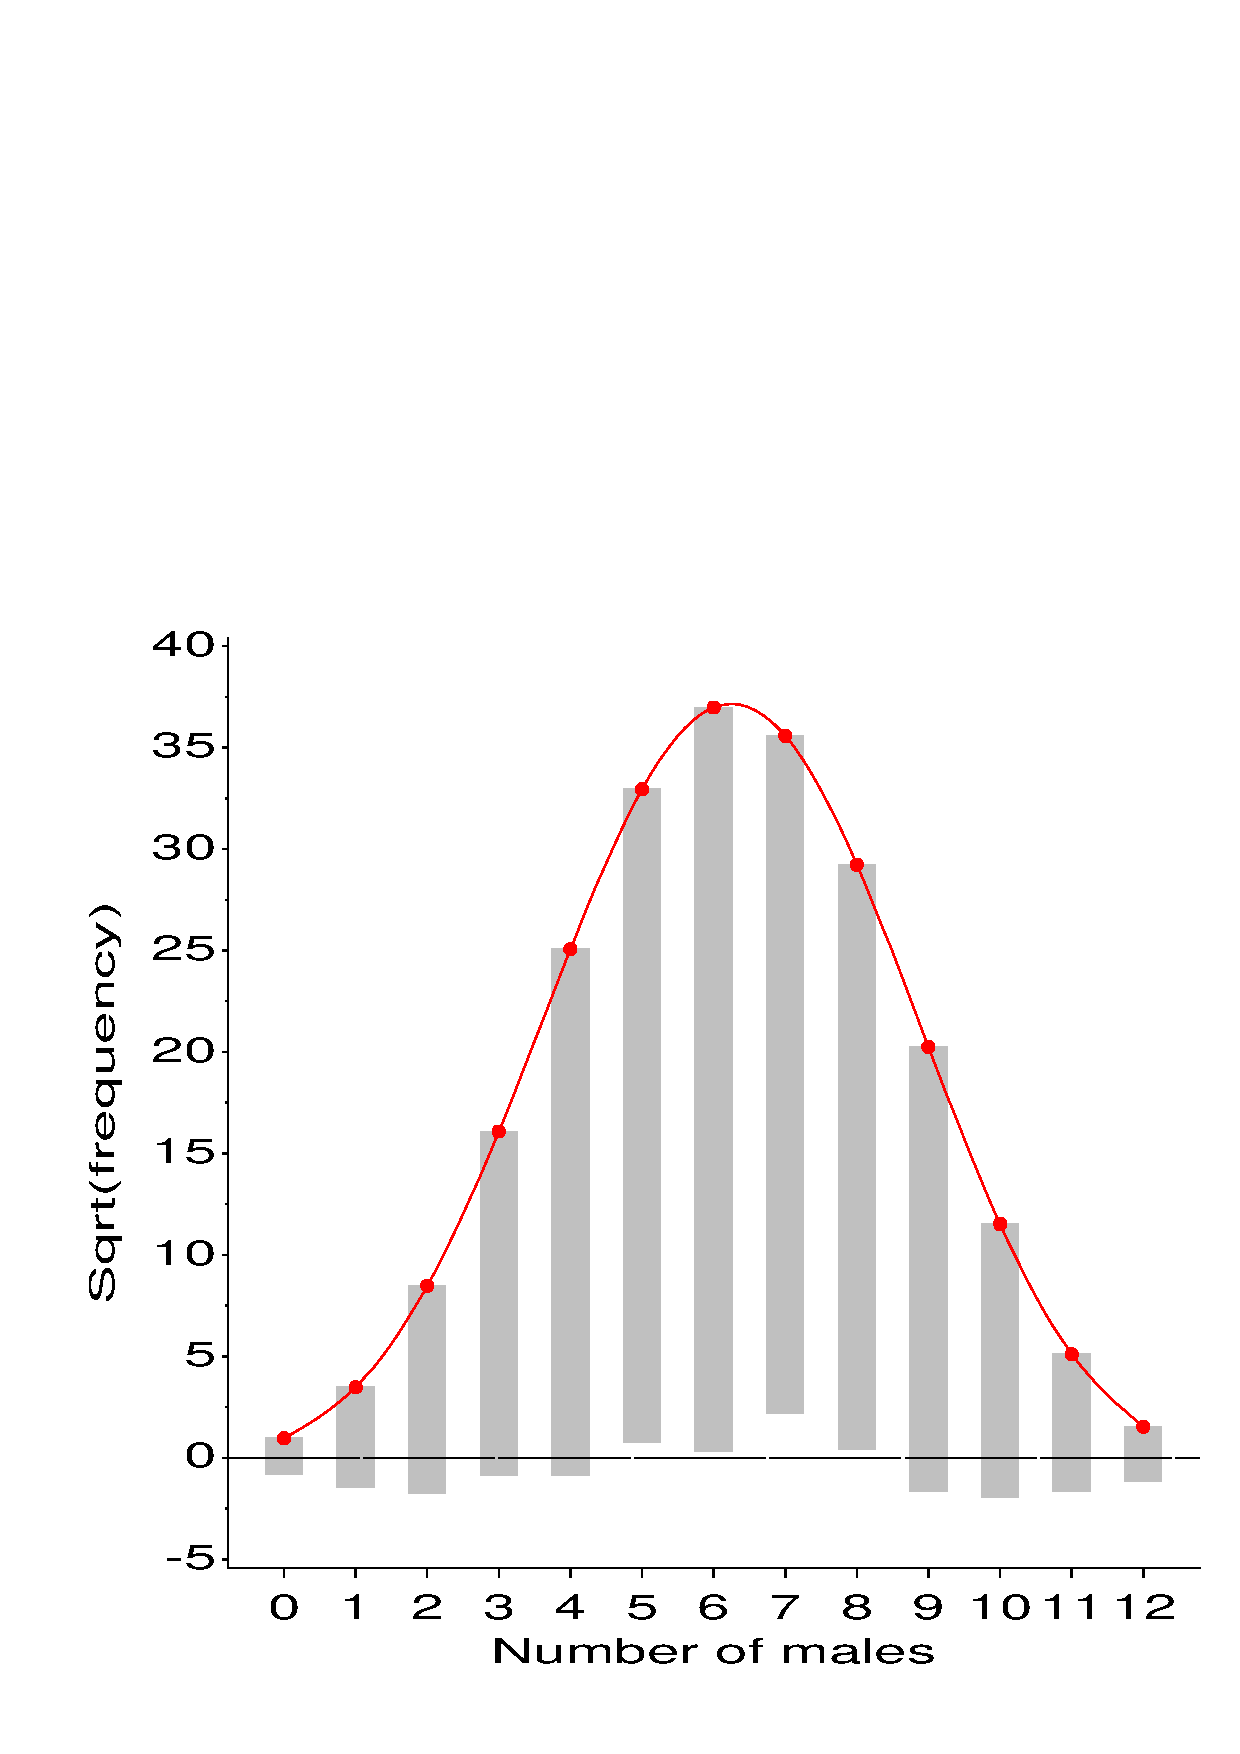
\includegraphics[width=1\linewidth]{saxony}\graphicsfile{ch2/fig/saxony.eps}{}
 \end{minipage}%
 \hfill
 \begin{minipage}[c]{.33\linewidth}
  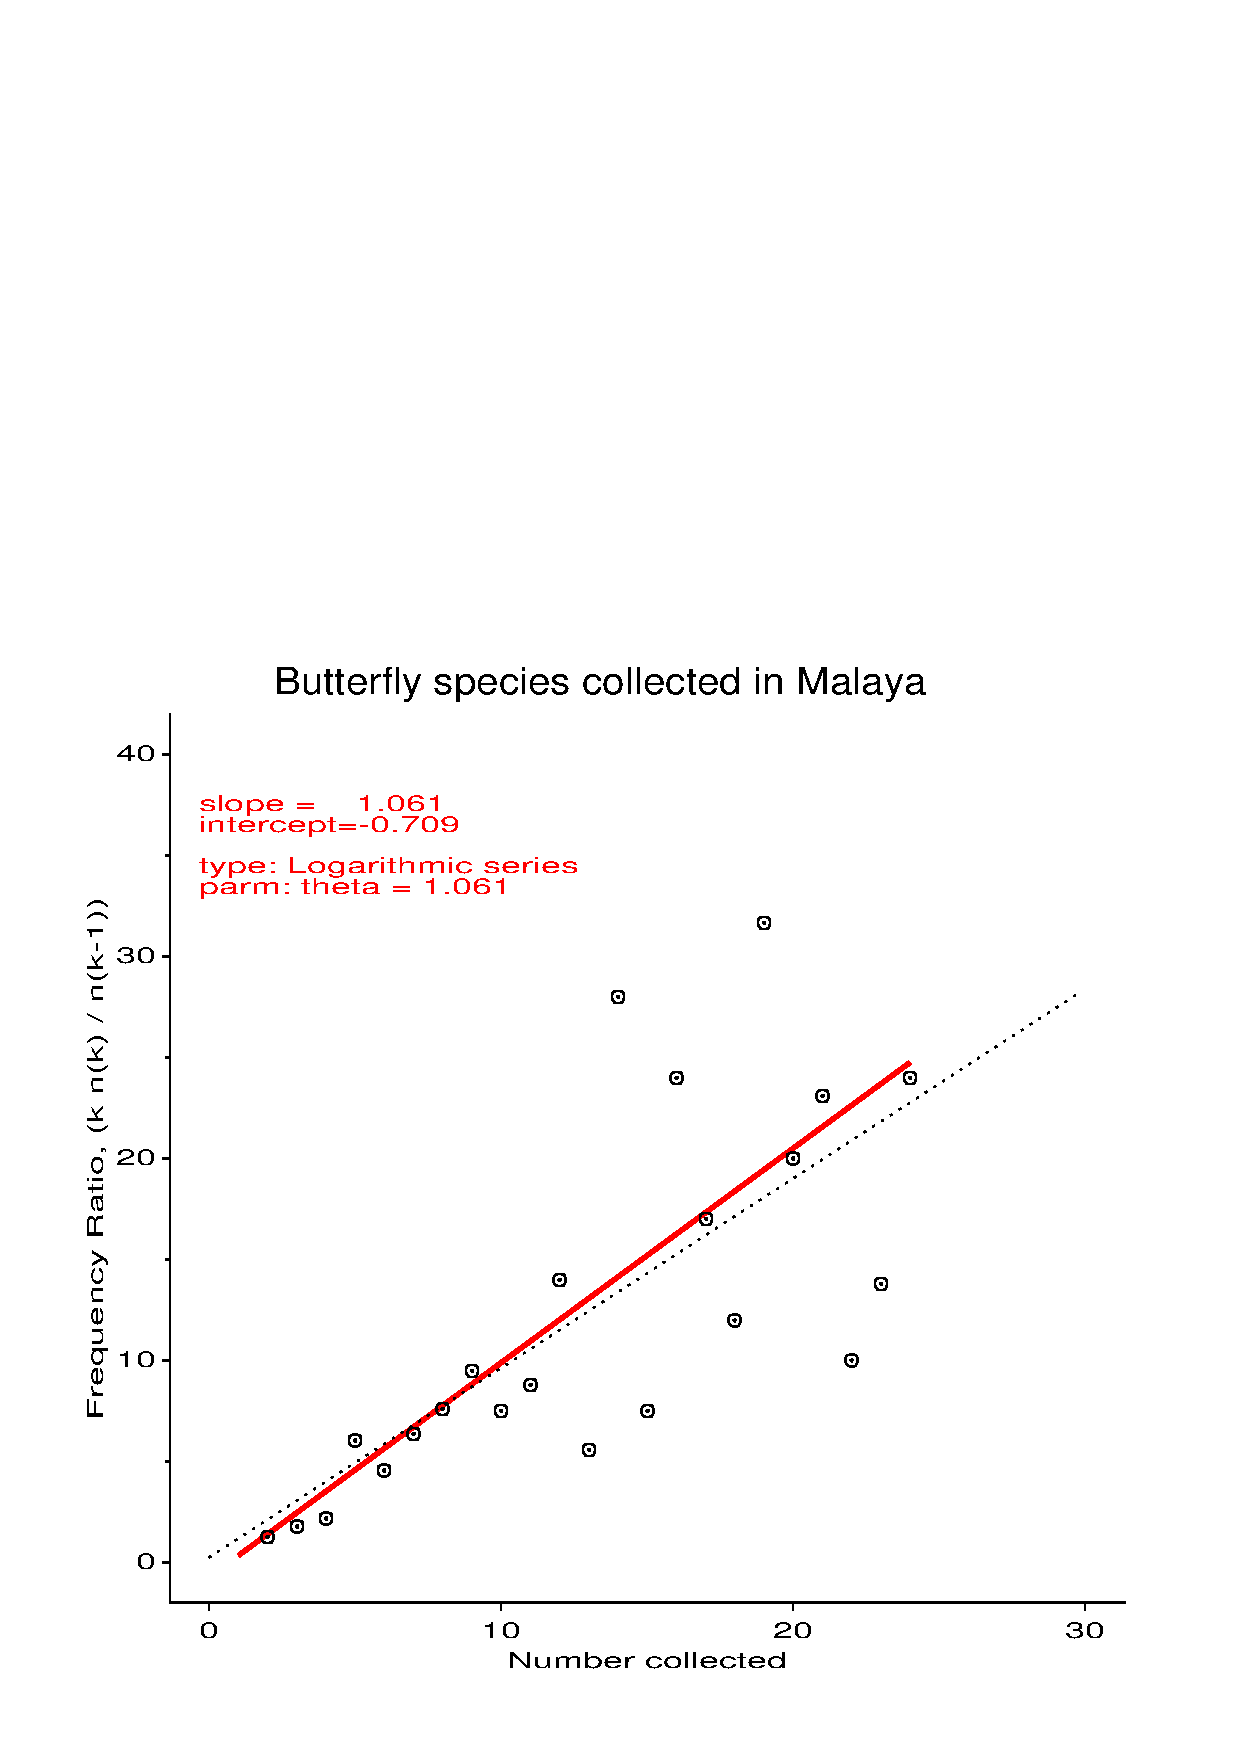
\includegraphics[width=1\linewidth]{orddemo3}\graphicsfile{ch2/fig/orddemo3.eps}{}
 \end{minipage}
 \hfill
 \begin{minipage}[c]{.33\linewidth}
  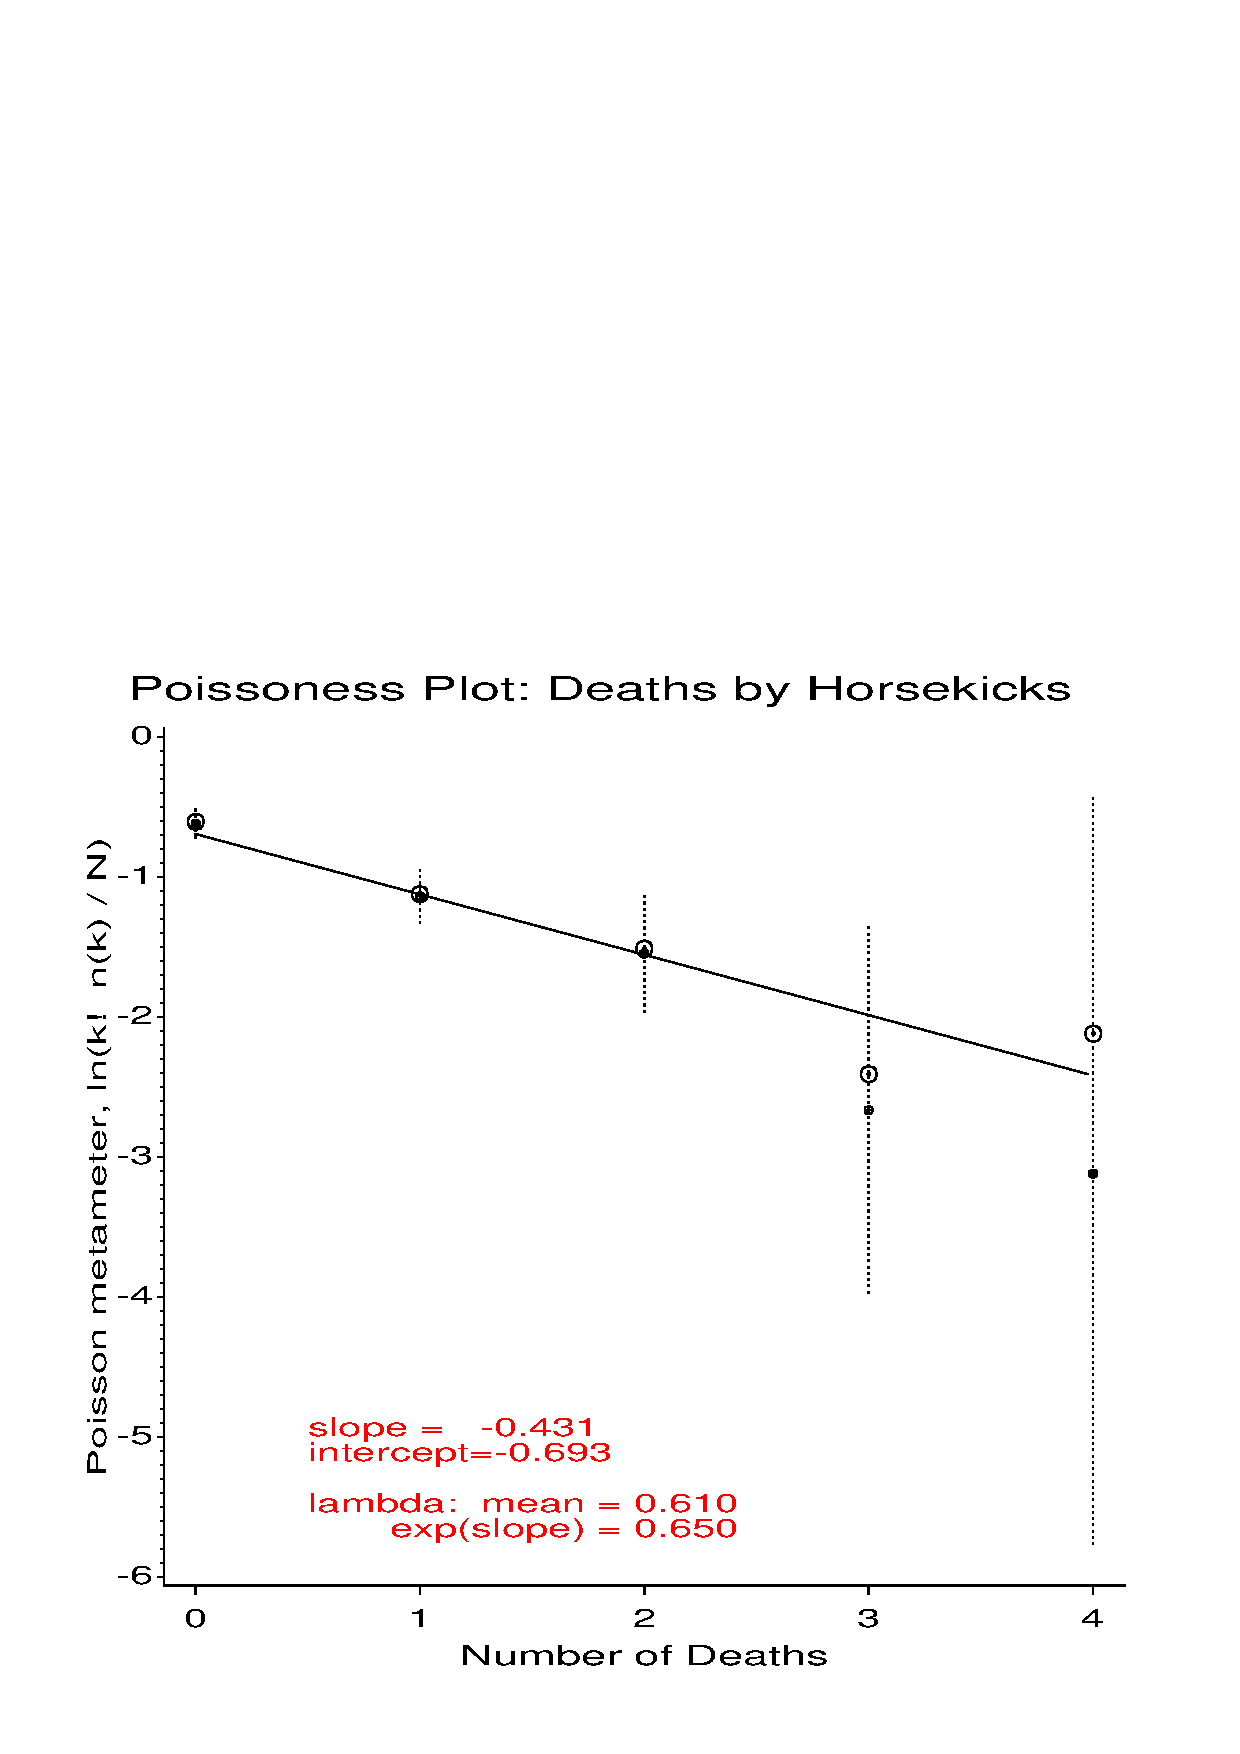
\includegraphics[width=1\linewidth]{poisdemo1}\graphicsfile{ch2/fig/poisdemo1.eps}{}
 \end{minipage}
\end{center}

		% visual table of contents

\chapterprelude{
Generalized linear models extend the familiar linear models of
regression and ANOVA to
include counted data, frequencies, and other data for which the
assumptions of independent, normal errors are not reasonable.
We rely on the analogies between ordinary and generalized linear
models (GLMs) to develop visualization methods to display the fitted
relations and check model assumptions.
}
% \minitoc
% \clearpage

\epigraph{In one word, to draw the rule from experience, one must generalize; this is a necessity that imposes itself on the most circumspect observer.}
{Henri Poincar\'e, \emph{The Value of Science: Essential Writings of Henri Poincare}}

In the modern history of statistics, most developments occur incrementally, with
small additions to existing models and theory that extend their range
and applicability to new problems and data.  Occasionally, there is
a major synthesis that unites a wide class of existing methods in a
general framework and provides opportunities for far greater growth.

A prime example is the theory of generalized linear models, introduced
originally by \citet{NelderWedderburn:72}, that extended the familiar
(classical) linear models for regression and ANOVA to include related
models, such as logistic regression and logit models (described in \chref{ch:logistic})
and \loglin models (described in \chref{ch:loglin})
and other variations as ``families'' within a single general system.

This approach has proved attractive because it:
\begin{seriate}
 \item integrates many familiar statistical models in a general theory where they are
 just special cases;
 \item provides the basis for extending these and developing new models within the
 same framework;
 \item simplifies the implementation of these models in software, since the same
 algorithm can be used for estimation, inference and assessing model adequacy
 for all generalized linear models.
\end{seriate}

\secref{glm:components} gives a brief sketch of the GLM framework.
The focus of this book is on visualization methods for categorical
data, and the two important topics concern models and methods for binomial response data
and for count data.  The first of these, 
was described extensively in
\chref{ch:logistic}, 
with extensions to multinomial
data (\secref{sec:logist-poly})
% and multivariate responses
and there is little to add here, except for changes
in notation.

GLM models for count data, however, provide the opportunity to extend 
the scope of of these methods beyond what was covered in \chref{ch:loglin},
and this topic is introduced in \secref{sec:glm-count}.
The GLM framework also provides the opportunity to deal with common problems
of overdispersion (\secref{sec:glm-overdisp}) and an overabundance of
zero counts (\secref{sec:glm-overdisp}), giving some new models and
visualization methods that help to understand such data in greater detail.
\secref{sec:glm-diag} illustrates other graphical methods for diagnostic
model checking, some of which were introduced in earlier chapters.
\TODO{Complete this chapter overview.}



\section{Components of Generalized Linear Models}\label{glm:components}

The motivation for the \term{generalized linear model} (GLM) and its structure are most
easily seen by considering the classical linear model,
\begin{equation*}
y_i = \vec{x}_i\trans \vec{\beta} + \epsilon_i
\end{equation*}
where 
$y_i$ is the response variable for case $i, i=1, \dots n$,
$\vec{x}_i$ is the vector of explanatory variables or regressors, 
$\vec{\beta}$ is the vector of model parameters, and the
$\epsilon_i$ are random errors.
In the classical linear model, the $\epsilon_i$ are assumed to
\begin{seriate}
  \item have constant variance, $\sigma^2_\epsilon$,
  \item follow a normal (Gaussian) distribution (conditional on $\vec{x}_i$),
  \item be independent across observations.
\end{seriate}

Thus, \citet{NelderWedderburn:72} generalized this gaussian linear model to
consist of the following three components, by relaxing assumptions (a) and (b) above:%
\footnote{The remaining assumption of independent observations is relaxed in
\term{generalized linear mixed models} (GLMMs), in which random effects to account for non-independence
are added to the linear predictor.
This allows the modeling of correlated (responses of family members), clustered (residents in 
different communities)
or hierarchical data
(patients within hospitals within regions). See: \citet{McCullochNeuhaus:2005} ...
\TODO{other references?}
}

\begin{description}
  \item[random component] The conditional distribution of the $y_i \given \vec{x}_i$,
  with mean $\E (y_i) = \mu_i$. Under classical assumptions,
  this is independent, normal with constant variance $\sigma^2$, i.e.,
  $ y_i \stackrel{\textrm{iid}}{\sim} N (\mu_i, \sigma^2)$.
  In the GLM, the probability distribution of the $y_i$ can be any member of the 
  \term{exponential family}, including the normal, Poisson, binomial, gamma
  and others. Subsequent work has extended this framework to include
  multinomial distributions and some non-exponential families such as the
  negative binomial distribution.
  
  
  \item[systematic component] The idea that the predicted value of $y_i$ itself
  is a linear
  combination of the regressors is replaced by that of a \term{linear predictor},
  $\eta$, that captures this aspect of linear models,
\begin{equation*}
\eta_i = \vec{x}_i\trans \vec{\beta}
\end{equation*}
  
  
  \item[link function] The connection between the mean of the the response, $\mu_i$,
  and the linear predictor, $\eta_i$, is specified by the \term{link function},
  $g(\bullet)$, giving
\begin{equation*}
g(\mu_i) = \eta_i = \vec{x}_i\trans \vec{\beta}
\end{equation*}
  The link function $g(\bullet)$ must be both \emph{smooth} and \emph{monotonic}, meaning that
  it is one-to-one, so an inverse transformation, $g^{-1}(\bullet)$ exists, 
\begin{equation*}
\mu_i = g^{-1}(\eta_i) = g^{-1}(\vec{x}_i\trans \vec{\beta})
\end{equation*}
  which allows us to obtain and plot the predicted values on their original scale.  The link function
  captures the familiar idea that linear models are often estimated with a transformation
  of the response, such as $\log(y_i)$ for a frequency variable or $\logit(y_i)$
  for a binomial variable.  The inverse function $g^{-1}(\bullet)$ 
  is also called the \term{mean function}. 
\end{description}

\begin{table}[htb]
\centering
\caption{Common link functions and their inverses used in generalized linear models}\label{tab:link-funcs}
\medskip
\renewcommand{\arraystretch}{1.25}
\begin{tabular}{lll}
\hline
%\rowcolor[gray]{.85}
\tableheader
Link name      & Function: $\eta_i = g(\mu_i)$ & Inverse: $\mu_i=g^{-1}(\eta_i)$  \\ \hline
identity       & $\mu_i$                       & $\eta_i$                      \\
square-root    & $\sqrt{\mu_i}$                & $\eta_i^2$                    \\
log            & $\log_e(\mu_i)$               & $\exp(\eta_i)$                \\ 
inverse        & $\mu_i^{-1}$                  & $\eta_i^{-1}$                 \\
inverse-square & $\mu_i^{-2}$                  & $\eta_i^{-1/2}$               \\ 
\hline
logit          & $\log_e\frac{\mu_i}{1-\mu_i}$ & $\frac{1}{1+\exp(-\eta_i)}$   \\
probit         & $\Phi^{-1}(\mu_i)$            & $\Phi^{-1}(\eta_i)$           \\
log-log        & $-\log_e[-\log_e(\mu_i)]$     & $\exp[-\exp(-\eta_i)]$        \\
comp. log-log  & $\log_e[-\log_e(1-\mu_i)]$    & $1-\exp[-\exp(\eta_i)]$       \\  \hline
\end{tabular}
\end{table}

Some commonly used link functions are shown in \tabref{tab:link-funcs}.
Some of these link functions have restrictions on the range of $y_i$
to which they can be applied.  For example, the square-root and log links
apply only to non-negative and
positive values respectively.  
The last four link functions in this
table are for binomial data, where $y_i$ represents the observed proportion
of successes in $n_i$ independent trials, and thus the mean $\mu_i$
represents the probability of success (symbolized by $\pi_i$ in \chref{ch:logistic}).
Binary data are the special case where $n_i=1$.

\subsection{Variance functions}
The GLM has the additional property that, for distributions in the exponential family,
the conditional variance of $y_i \given \eta_i$ is a known function, $\V (\mu_i)$
of the mean and possibly one other parameter called the \term{scale parameter} or
\term{dispersion parameter}, $\phi$. Some commonly used distributions in the 
exponential family and their variance functions are shown in \tabref{tab:exp-families}.

% Please add the following required packages to your document preamble:
% \usepackage[table,xcdraw]{xcolor}
% If you use beamer only pass "xcolor=table" option, i.e. \documentclass[xcolor=table]{beamer}
\begin{table}[htb]
\centering
\caption{Common distributions in the exponential family used with generalized linear models and their canonical link and variance functions}
\label{tab:exp-families}
\medskip
\renewcommand{\arraystretch}{1.25}
\begin{tabular}{lllll}
\hline
%\rowcolor[gray]{.85}
\tableheader
Family           & Notation          & Canonical link         & Range of $y$          & Variance function, $\V(\mu \given \eta)$ \\
\hline
Gaussian         & $N(\mu,\sigma^2)$ & identity: $\mu$        & $(-\infty, +\infty)$   & $\phi$                       \\
Poisson          & $\Pois(\mu)$      & $\log_e(\mu)$          & $0, 1, \dots, \infty$  & $\mu$                        \\
Negative-Binomial & $\NBin(\mu,\theta)$   & $\log_e(\mu)$     & $0, 1, \dots, \infty$ & $\mu + \mu^2/\theta$          \\
Binomial         & $\Bin(n,\mu)/n$   & $\logit(\mu)$          & $\{0, 1, \dots, n\}/n$ & $\mu (1-\mu)/n$              \\
Gamma            & $G(\mu, \nu)$     & $\mu^{-1}$             & $(0, +\infty)$         & $\phi \mu^2$                 \\
Inverse-Gaussian & $IG(\mu, \nu)$    & $\mu^2$                & $(0, +\infty)$         & $\phi \mu^3$                 \\
\hline
\end{tabular}
\end{table}

\begin{itemize}
\item In the classical Gaussian linear model, the conditional variance is constant,
$\phi = \sigma^2_\epsilon$. 

\item In the Poisson family, $\V (\mu_i) = \mu_i$
and the dispersion parameter is fixed at $\phi = 1$.
In practice, it is common for count data to exhibit \term{overdispersion},
meaning that $\V (\mu_i) > \mu_i$.  One way to correct for this is to extend
the GLM to allow the dispersion parameter to be estimated from the data,
giving what is called the \term{quasi-poisson} family, with $\V (\mu_i) = \widehat{\phi} \mu_i$.

\item Similarly, for binomial data, the variance function is $\V (\mu_i) = \mu_i (1-\mu_i) / n_i$,
with $\phi$ fixed at 1.
Overdispersion often results from failures of the assumptions of the binomial model:
supposedly independent observations may be correlated or clustered and the probability
of success may not be constant, or vary with unmeasured or unmodeled variables.

\item The gamma and inverse-Gaussian families are distributions useful for modeling a continuous
and positive response variable with no upper bound (e.g., reaction time). They both have the 
property that conditional variance increases with the mean, and for the inverse-Gaussian,
variance increases at a faster rate.  Their dispersion parameters $\phi$ are simple functions
of their intrinsic ``shape'' parameters, indicated as $\nu$ in the table.  

\end{itemize}

The important points from this discussion are that the GLM together with the exponential
family of distributions:
\begin{itemize}
 \item provide for simple, linear relations between the response and the predictors
 via the link function and the linear predictor.
 \item allows a very flexible relationship between the mean and 
 conditional variance to be specified in terms of a set of known families.
 \item incorporates a dispersion parameter $\phi$ that in some cases can be estimated
 or tested for departure from that entailed in a given family.
 \item has allowed further extensions of this framework outside the exponential family,
 ranging from simple adjustments for statistical inference (``quasi'' families, 
 adjusted ``sandwich'' covariances) to separate modeling of the variance relation
 to the predictors.
\end{itemize}

Further details of generalized linear models are beyond the scope of this book, but
the interested reader should consult \citet[\S 15.3]{Fox:2008} 
and \citet[Ch. 4]{Agresti:2013} for a comprehensive
treatment.

\subsection{Hypothesis tests for coefficients}
GLMs are fit using maximum likelihood estimation, and implemented in software using
an iterative algorithm known as \emph{iteratively weighted least squares}
that generalizes the least squares method for classical linear models.
This provides estimates $\vec{\widehat{\beta}}$ of the model coefficients
for the predictors in $\vec{x}$, as well as an estimated asymptotic 
(large sample) variance matrix of $\vec{\widehat{\beta}}$, given by
\begin{equation}\label{eq:varbeta}
\V (\widehat{\vec{\beta}}) = \phi ( \mat{X}\trans  \mat{W} \mat{X} )
\end{equation}
where $\mat{W}$ is a diagonal matrix of weights computed in the final iteration.
In the standard Poisson GLM, the weight matrix is $\mat{W} = \diag (\widehat{\vec{\mu}})$
and $\phi=1$ is assumed.

Asymptotic standard errors, $ se (\widehat{\beta}_j)$,
for the coefficients are then the square roots of the
diagonal elements
% $ \sqrt{ \V (\widehat{\vec{\beta}})_{jj}}$,
of $\V (\widehat{\beta})$, and tests of hypotheses regarding
an individual coefficient, e.g., $H_0 : \beta_j = 0$, can be carried out
using the Wald test statistic,
$z_j = \widehat{\beta}_j / se (\widehat{\beta}_j)$.
When the null hypothesis is true, $z_j$ has a standard normal $N(0,1)$
distribution, providing $p$-values for significance tests.%
\footnote{Wald tests are sometimes carried out using $z^2$, which has an equivalent
$\chi^2_1$ distribution with 1 degree of freedom.
}


\subsection{Goodness-of-fit tests}\label{sec:glm-goodfit}
The basic ideas for testing goodness-of-fit were discussed in \secref{sec:loglin-goodfit}
in connection with \loglin models for \ctabs.
As before, these assess the overall performance of a model in reproducing the data.
The commonly used measures include the Pearson chi-square and
\LR deviance statistics, which can be seen as weighted sums of residuals.
We re-state these test statistics here in the wider context of the GLM.

Let $y_i, i=1, 2, \dots, n$ be the response and $\widehat{\mu}_i = g^{-1} (\vec{x}_i\trans \widehat{\vec{\beta}})$
the fitted mean using the estimated coefficients, having estimated variance
$\widehat{\omega}_i = \V(\widehat{\mu}_i\given \eta_i)$ as in \tabref{tab:exp-families}.
Then the normalized squared residual for observation $i$ is
$(y_i - \widehat{\mu}_i)^2 / \widehat{\omega}_i$, and the Pearson statistic is
\begin{equation}\label{eq:pearson}
X^2_P = \sum_{i=1}^n \frac{(y_i - \widehat{\mu}_i)^2}{\widehat{\omega}_i} \period
\end{equation}

In the GLM for count data, the main focus of this chapter, the Poisson family
sets $\omega = \mu$ with the dispersion parameter fixed at $\phi=1$.

The \term{residual deviance} statistic, as in logistic regression and \loglin models
is defined as twice the difference between the maximum possible log-likelihood
for the \emph{saturated model} that fits perfectly and maximized log-likelihood
for the fitted model. The deviance can be defined as
\begin{equation*}
D (\vec{y}, \vec{\widehat{\mu}}) \equiv 2 [ \log \mathcal{L}(\vec{y};\vec{y}) - \log \mathcal{L}(\vec{y};\vec{\widehat{\mu}})]
\end{equation*}
For classical linear models under normality, the deviance is simply the residual sum of squares,
$\sum_i^n (y_i - \widehat{\mu}_i)$.  This has led to the deviance being taken in the GLM
framework as a generalization of the sum of squares used in ANOVA, and hence, an anlogous
\term{analysis of deviance} to carry out tests for individual terms in GLMs, or to compare
nested models.  

In \R, \code{anova(mod)} for the \class{glm} object \code{mod}
gives \emph{sequential} (``Type I'') tests of successive terms in a model, while
\func{Anova} in the \Rpackage{car} gives the more generally useful 
``Type II'' (and ``Type III'') \emph{partial} tests, that assess the additional
contribution of each term above all others, taking marginality into account.

For Poisson models with a log link giving $\vec{\mu} = \exp(\vec{x}\trans \vec{\beta})$ , the deviance takes the form%
\footnote{In the context of the \loglin models discussed in \secref{sec:loglin-goodfit}, this is also referred to
as the \LR $G^2$ statistic.}

\begin{equation}\label{eq:pois-deviance}
D (\vec{y}, \vec{\widehat{\mu}}) = 
  2 \sum_{i=1}^n \left[ y_i \log_e \left( \frac{y_i}{\widehat{\mu}_i} \right) - (y_i - \widehat{\mu}_i) \right]
\end{equation}
For a GLM with $p$ parameters, both the Pearson and residual deviance statistics follow
approximate $\chi^2_{n-p}$ distributions with $n-p$ degrees of freedom.

% \section{GLMs for binomial data}\label{sec:glm-binomial}
% 
% \TODO{Don't need to include this, because these models were extensively treated in \chref{ch:logistic}.}

\section{GLMs for count data}\label{sec:glm-count}

%\section{GLMs for count data}\label{sec:glm-count}

The prototypical GLM for count data, where the response $y_i$
takes on non-negative values $0, 1, 2, \dots$, 
uses the Poisson family with the log link.
We used this model extensively throughout all of \chref{ch:loglin}.
There the focus was on the special case of the \loglin model
applied largely to contingency tables, where the \loglin model could
be seen as a fairly direct extension of ANOVA models for a 
quantitative response applied to the log of cell frequency.

The advantage there was that models for two-way, three-way and 
by implication \nway tables could be discussed and illustrated
using notation and graphs that separated the parameters and
effects for one-way terms (``main effects''), two-way terms
(``simple associations'') and higher-way terms (``conditional associations'').

The disadvantage is that these models as formulated there do not
easily accommodate general quantitative predictors and
were limited to the log link and the Poisson family.
For example, the models discussed in \secref{sec:loglin-ordinal}
for ordinal variables allow one or more table factors to be
assigned quantitative scores or have such scores estimated from
the data, as in RC() models (\secref{sec:RCmodels}).
Yet, the \ctab approach for \loglin models breaks down if there are
continuous predictors, and count data often exhibits features that
make the equivalent Poisson regression model unsuitable or incomplete.
We consider some extended models here.


\begin{Example}[phdpubs1]{Publications of PhD candidates}
In \exref{ex:phdpubs0} we considered the distribution of the number of 
publications by PhD candidates in their last three years of study,
but without taking any available predictors into account. 
For these data, a simple calculation shows why the Poisson distribution
is unsuitable (for the marginal distribution), because the variance is 2.19 times the mean.

\begin{knitrout}
\definecolor{shadecolor}{rgb}{1, 0.961, 0.933}\color{fgcolor}\begin{kframe}
\begin{alltt}
\hlkwd{data}\hlstd{(}\hlstr{"PhdPubs"}\hlstd{,} \hlkwc{package}\hlstd{=}\hlstr{"vcdExtra"}\hlstd{)}
\hlkwd{with}\hlstd{(PhdPubs,} \hlkwd{c}\hlstd{(}\hlkwc{mean}\hlstd{=}\hlkwd{mean}\hlstd{(articles),} \hlkwc{var}\hlstd{=}\hlkwd{var}\hlstd{(articles),}
                \hlkwc{ratio}\hlstd{=}\hlkwd{var}\hlstd{(articles)}\hlopt{/}\hlkwd{mean}\hlstd{(articles)))}
\end{alltt}
\begin{verbatim}
##  mean   var ratio 
## 1.693 3.710 2.191
\end{verbatim}
\end{kframe}
\end{knitrout}
The earlier example showed rootograms (in \figref{fig:phdpubs-rootogram})
of the number of articles, but here it is useful to consider some more
basic exploratory displays.  A basic barplot of the frequency distribution
of number of articles published is shown in the left panel of
\figref{fig:phdpubs-barplot}.  A quick look indicates that the distribution
is highly skewed and there is a large number of counts of zero.

Another problem is that the frequencies of 0--2 articles account for 
over 75\% of the total, so that the frequencies of the larger counts
get lost in the display.  The rootogram corrects for this by plotting
frequency on the square-root scale.  However, because we are contemplating
a model with a log link, the same goal can be achieved by ploting
log of frequency, as shown in the right panel of \figref{fig:phdpubs-barplot}.
To accommodate the zero frequencies, the plot shows log(Frequency+1),
avoiding errors from \code{log(0)}.
It can be seen that log frequency decreases steadily up to 7 articles and
then levels off approximately.

\begin{figure}[htb]
  \centering
  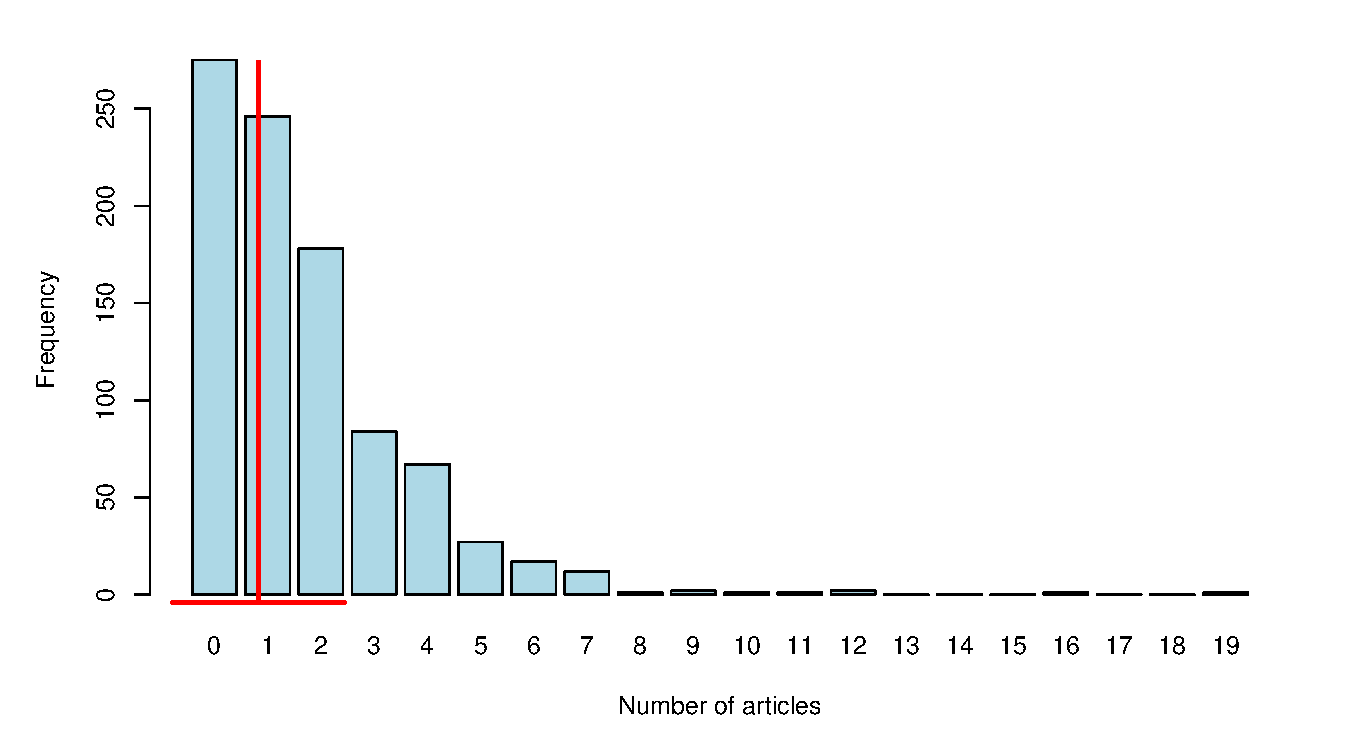
\includegraphics[width=.49\textwidth]{ch09/fig/phdpubs-barplot1}
  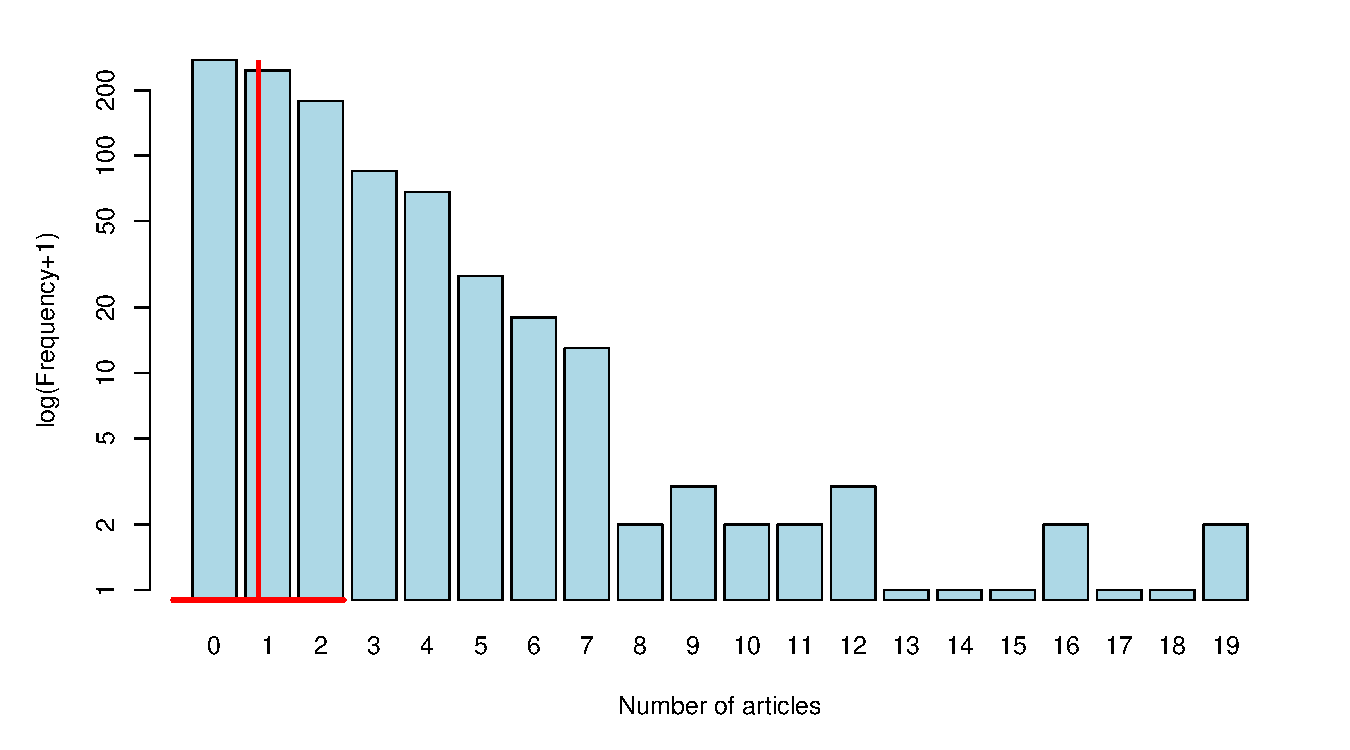
\includegraphics[width=.49\textwidth]{ch09/fig/phdpubs-barplot2}
  \caption{Barplots showing the frequency distribution of number of publications by PhD candidates.
  Left: raw scale; Right: a log scale makes the smaller counts more visible. The vertical red
  lines show the mean and horizontal lines show mean $\pm 1$  standard deviation.}
  \label{fig:phdpubs-barplot}
\end{figure}

These plots are produced as shown below.  The frequency distribution of
\code{articles} can be tabulated by \func{table}, but there is a subtle
wrinkle here:  By default, \func{table} excludes the values of \code{articles}
that do not occur in the data (zero frequencies).  To include all values in
the entire range, it is necessary to treat \code{articles} as a factor
with levels \code{0:19}.

\begin{knitrout}\footnotesize
\definecolor{shadecolor}{rgb}{1, 0.961, 0.933}\color{fgcolor}\begin{kframe}
\begin{alltt}
\hlstd{art.fac} \hlkwb{<-} \hlkwd{factor}\hlstd{(PhdPubs}\hlopt{$}\hlstd{articles,} \hlkwc{levels}\hlstd{=}\hlnum{0}\hlopt{:}\hlnum{19}\hlstd{)}  \hlcom{# include zero frequencies}
\hlstd{art.tab} \hlkwb{<-} \hlkwd{table}\hlstd{(art.fac)}
\hlstd{art.tab}
\end{alltt}
\begin{verbatim}
## art.fac
##   0   1   2   3   4   5   6   7   8   9  10  11  12  13  14  15  16  17  18  19 
## 275 246 178  84  67  27  17  12   1   2   1   1   2   0   0   0   1   0   0   1
\end{verbatim}
\end{kframe}
\end{knitrout}
Then, the basic plot on the frequency scale is created using \func{barplot},
and some annotations showing the mean and a one standard deviation interval
can be added using standard plotting tools.
\begin{knitrout}
\definecolor{shadecolor}{rgb}{1, 0.961, 0.933}\color{fgcolor}\begin{kframe}
\begin{alltt}
\hlkwd{barplot}\hlstd{(art.tab,} \hlkwc{xlab}\hlstd{=}\hlstr{"Number of articles"}\hlstd{,} \hlkwc{ylab}\hlstd{=}\hlstr{"Frequency"}\hlstd{,}
        \hlkwc{col}\hlstd{=}\hlstr{"lightblue"}\hlstd{)}
\hlkwd{abline}\hlstd{(}\hlkwc{v}\hlstd{=}\hlkwd{mean}\hlstd{(PhdPubs}\hlopt{$}\hlstd{articles),} \hlkwc{col}\hlstd{=}\hlstr{"red"}\hlstd{,} \hlkwc{lwd}\hlstd{=}\hlnum{3}\hlstd{)}
\hlstd{ci} \hlkwb{<-} \hlkwd{mean}\hlstd{(PhdPubs}\hlopt{$}\hlstd{articles)}\hlopt{+}\hlkwd{c}\hlstd{(}\hlopt{-}\hlnum{1}\hlstd{,}\hlnum{1}\hlstd{)} \hlopt{*} \hlkwd{sqrt}\hlstd{(}\hlkwd{var}\hlstd{(PhdPubs}\hlopt{$}\hlstd{articles))}
\hlkwd{lines}\hlstd{(}\hlkwc{x}\hlstd{=ci,} \hlkwc{y}\hlstd{=}\hlkwd{c}\hlstd{(}\hlopt{-}\hlnum{4}\hlstd{,} \hlopt{-}\hlnum{4}\hlstd{),} \hlkwc{col}\hlstd{=}\hlstr{"red"}\hlstd{,} \hlkwc{lwd}\hlstd{=}\hlnum{3}\hlstd{,} \hlkwc{xpd}\hlstd{=}\hlnum{TRUE}\hlstd{)}
\end{alltt}
\end{kframe}
\end{knitrout}

Similarly, the plot on the log scale in the right panel of \figref{fig:phdpubs-barplot}
is produced with \func{barplot}, but using \code{art.tab+1} to start frequency at one
and \code{log="y"} to scale the vertical axis to log.

\begin{knitrout}
\definecolor{shadecolor}{rgb}{1, 0.961, 0.933}\color{fgcolor}\begin{kframe}
\begin{alltt}
\hlkwd{barplot}\hlstd{(art.tab}\hlopt{+}\hlnum{1}\hlstd{,} \hlkwc{ylab}\hlstd{=}\hlstr{"log(Frequency+1)"}\hlstd{,} \hlkwc{xlab}\hlstd{=}\hlstr{"Number of articles"}\hlstd{,}
        \hlkwc{col}\hlstd{=}\hlstr{"lightblue"}\hlstd{,} \hlkwc{log}\hlstd{=}\hlstr{"y"}\hlstd{)}
\end{alltt}
\end{kframe}
\end{knitrout}
Other useful exploratory plots for count data include boxplots of the response (on a log scale)
and scatterplots against continuous predictors, where jittering the response is often
necessary to avoid overplotting and a smooth nonparametric curve can show possible non-linearity.
The \code{log="y"} option is again handy, and the formula
method allows adding a start value to the response.  \figref{fig:phdpubs-logplots}
illustrates these ideas, for the factor \code{married} and the covariate \code{mentor}.
\begin{knitrout}
\definecolor{shadecolor}{rgb}{1, 0.961, 0.933}\color{fgcolor}\begin{kframe}
\begin{alltt}
\hlkwd{boxplot}\hlstd{(articles}\hlopt{+}\hlnum{1} \hlopt{~} \hlstd{married,} \hlkwc{data}\hlstd{=PhdPubs,} \hlkwc{log}\hlstd{=}\hlstr{"y"}\hlstd{,} \hlkwc{varwidth}\hlstd{=}\hlnum{TRUE}\hlstd{,}
        \hlkwc{ylab}\hlstd{=}\hlstr{"log(articles+1)"}\hlstd{,} \hlkwc{xlab}\hlstd{=}\hlstr{"married"}\hlstd{,} \hlkwc{cex.lab}\hlstd{=}\hlnum{1.25}\hlstd{)}
\hlkwd{plot}\hlstd{(}\hlkwd{jitter}\hlstd{(articles}\hlopt{+}\hlnum{1}\hlstd{)} \hlopt{~} \hlstd{mentor,} \hlkwc{data}\hlstd{=PhdPubs,} \hlkwc{log}\hlstd{=}\hlstr{"y"}\hlstd{,}
      \hlkwc{ylab}\hlstd{=}\hlstr{"log(articles+1)"}\hlstd{,} \hlkwc{cex.lab}\hlstd{=}\hlnum{1.25}\hlstd{)}
\hlkwd{lines}\hlstd{(}\hlkwd{lowess}\hlstd{(PhdPubs}\hlopt{$}\hlstd{mentor, PhdPubs}\hlopt{$}\hlstd{articles}\hlopt{+}\hlnum{1}\hlstd{),} \hlkwc{col}\hlstd{=}\hlstr{"red"}\hlstd{,} \hlkwc{lwd}\hlstd{=}\hlnum{2}\hlstd{)}
\end{alltt}
\end{kframe}\begin{figure}[!htbp]


\centerline{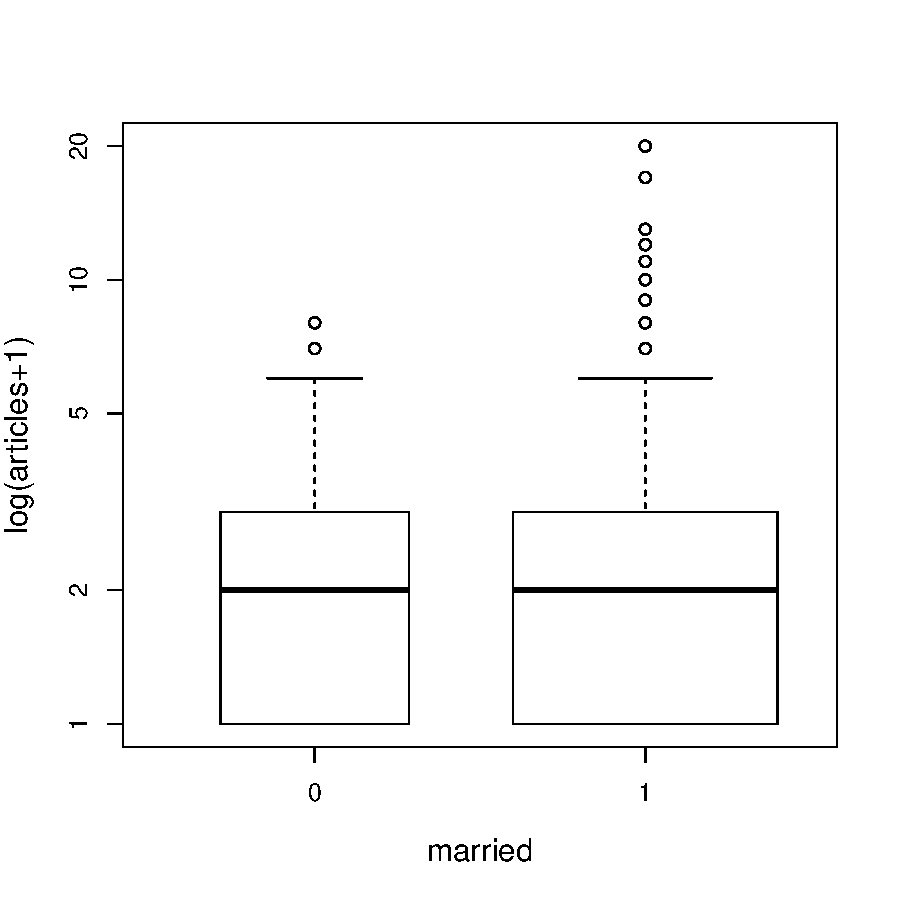
\includegraphics[width=.49\textwidth]{ch09/fig/phdpubs-logplots1} 
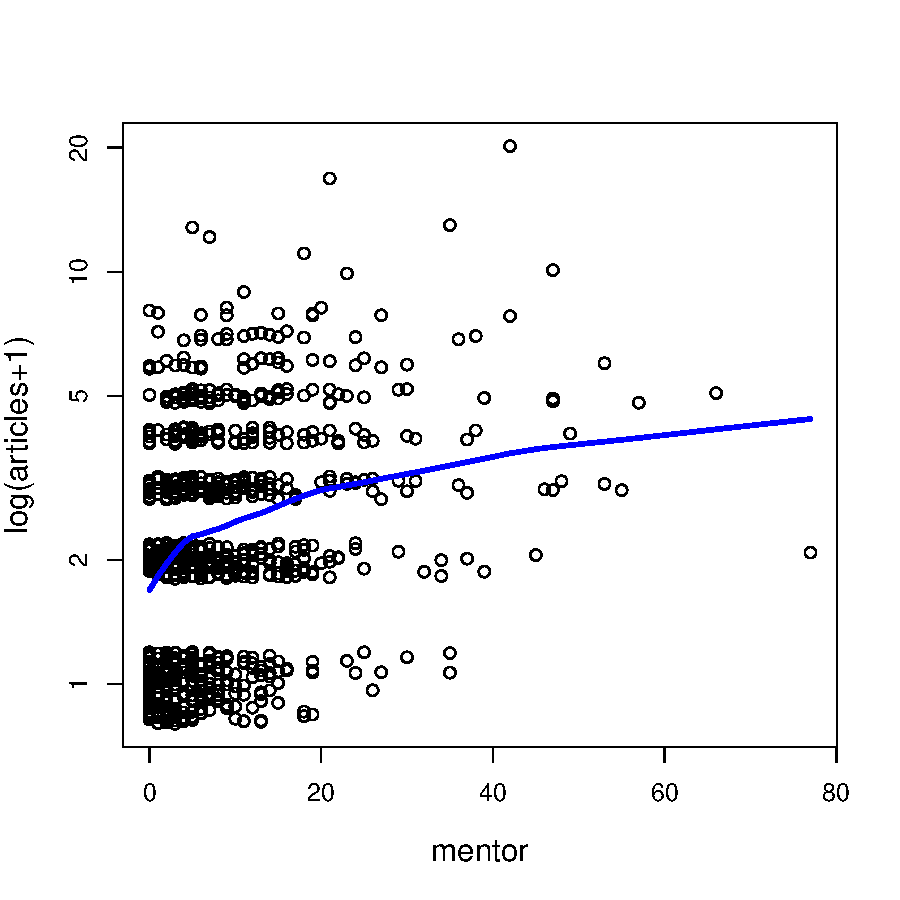
\includegraphics[width=.49\textwidth]{ch09/fig/phdpubs-logplots2} }

\caption[Exploratory plots for the number of articles in the PhdPubs data]{Exploratory plots for the number of articles in the PhdPubs data. Left: boxplots for married (1) vs. non-married (0); right: jittered scatterplot vs. mentor publicationswith a lowess smoothed curve.\label{fig:phdpubs-logplots}}
\end{figure}


\end{knitrout}
It can be seen that the distribution of articles for married and non-married are quite similar,
except that for the married students there are quite a few observations with a large number
of publications.  The relationship between log(articles) and mentor publications seems largely
linear except possibly at the very low end.  The large number of zero counts at the lower left
corner stands out; this would not be seen without jittering.

To start analysis, we fit the Poisson model using all predictors---
\code{female}, \code{married}, \code{kid5}, \code{phdprestige}, and
\code{mentor}. As recorded in \data{PhdPubs}, \code{female} and
\code{married} are both dummy (0/1) variables, and it it slightly
more convenient for plotting purposes to make them factors.

\begin{knitrout}
\definecolor{shadecolor}{rgb}{1, 0.961, 0.933}\color{fgcolor}\begin{kframe}
\begin{alltt}
\hlstd{PhdPubs} \hlkwb{<-} \hlkwd{within}\hlstd{(PhdPubs, \{}
  \hlstd{female} \hlkwb{<-} \hlkwd{factor}\hlstd{(female)}
  \hlstd{married} \hlkwb{<-} \hlkwd{factor}\hlstd{(married)}
\hlstd{\})}
\end{alltt}
\end{kframe}
\end{knitrout}

The model is fit as shown below and summarized using \func{summary}, but with abbreviated output.
\begin{knitrout}
\definecolor{shadecolor}{rgb}{1, 0.961, 0.933}\color{fgcolor}\begin{kframe}
\begin{alltt}
\hlstd{phd.pois} \hlkwb{<-} \hlkwd{glm}\hlstd{(articles} \hlopt{~} \hlstd{.,} \hlkwc{data}\hlstd{=PhdPubs,} \hlkwc{family}\hlstd{=poisson)}
\hlkwd{summary}\hlstd{(phd.pois)}
\end{alltt}
\begin{verbatim}
...
## Coefficients:
##             Estimate Std. Error z value Pr(>|z|)    
## (Intercept)  0.26562    0.09962    2.67   0.0077 ** 
## female1     -0.22442    0.05458   -4.11  3.9e-05 ***
## married1     0.15732    0.06125    2.57   0.0102 *  
## kid5        -0.18491    0.04012   -4.61  4.0e-06 ***
## phdprestige  0.02538    0.02527    1.00   0.3153    
## mentor       0.02523    0.00203   12.43  < 2e-16 ***
## ---
## Signif. codes:  0 '***' 0.001 '**' 0.01 '*' 0.05 '.' 0.1 ' ' 1
## 
## (Dispersion parameter for poisson family taken to be 1)
## 
##     Null deviance: 1817.4  on 914  degrees of freedom
## Residual deviance: 1633.6  on 909  degrees of freedom
## AIC: 3313
...
\end{verbatim}
\end{kframe}
\end{knitrout}
Significance tests for the individual coefficients show that all are significant,
except for \code{phdprestige}.  We ignore this here, and continue to interpret and
extend the full main effects model.%
\footnote{
It is usually less harmful to include a non-significant predictor,
(which in any case may be a variable useful to control, as \code{phdprestige} here), than to omit a
potentially important predictor, or worse--- to fail to account for an important interaction.
}

The estimated coefficients $\vec{\beta}$ for the predictors are shown below.
Recall that using the log link means, for example, that being married increases
the log of the expected number of
articles published by 0.157, holding all other predictors constant. 
Each additional child of age 5 or less decreases this by 0.185.
\begin{knitrout}
\definecolor{shadecolor}{rgb}{1, 0.961, 0.933}\color{fgcolor}\begin{kframe}
\begin{alltt}
\hlkwd{round}\hlstd{(}\hlkwd{cbind}\hlstd{(}\hlkwc{beta}\hlstd{=}\hlkwd{coef}\hlstd{(phd.pois),}
            \hlkwc{expbeta}\hlstd{=}\hlkwd{exp}\hlstd{(}\hlkwd{coef}\hlstd{(phd.pois)),}
            \hlkwc{pct}\hlstd{=}\hlnum{100}\hlopt{*}\hlstd{(}\hlkwd{exp}\hlstd{(}\hlkwd{coef}\hlstd{(phd.pois))}\hlopt{-}\hlnum{1}\hlstd{)),}\hlnum{3}\hlstd{)}
\end{alltt}
\begin{verbatim}
##               beta expbeta     pct
## (Intercept)  0.266   1.304  30.425
## female1     -0.224   0.799 -20.102
## married1     0.157   1.170  17.037
## kid5        -0.185   0.831 -16.882
## phdprestige  0.025   1.026   2.570
## mentor       0.025   1.026   2.555
\end{verbatim}
\end{kframe}
\end{knitrout}
\noindent It is somewhat easier to interpret the exponentiated coefficients, $\exp(\vec{\beta})$
as multiplicative effects on the expected number of articles and convert these to percentage
change, again holding other predictors constant.
For example, expected publications by married candidates are 1.17 times that of non-married,
a 17\% increase, while each additional child multiplies articles by 0.831, a 16.88\% decrease.

Alternatively, we recommend visual displays for model interpretation, and effect plots do well
in most cases, as shown in  \figref{fig:phdpubs1-effpois}.
For a Poisson GLM, an important feature is that the response is plotted on
the log scale, so that effects in the model appear as linear functions, while the
values of the response (numer of articles) are labeled on their original scale, facilitating
interpretation. The confidence bands and error bars give 95\% confidence intervals
around the fitted efffects.

\begin{knitrout}
\definecolor{shadecolor}{rgb}{1, 0.961, 0.933}\color{fgcolor}\begin{kframe}
\begin{alltt}
\hlkwd{library}\hlstd{(effects)}
\hlkwd{plot}\hlstd{(}\hlkwd{allEffects}\hlstd{(phd.pois),} \hlkwc{band.colors}\hlstd{=}\hlstr{"blue"}\hlstd{,} \hlkwc{lwd}\hlstd{=}\hlnum{3}\hlstd{,}
     \hlkwc{ylab}\hlstd{=}\hlstr{"Number of articles"}\hlstd{,} \hlkwc{main}\hlstd{=}\hlstr{""}\hlstd{)}
\end{alltt}
\end{kframe}\begin{figure}[!htbp]


\centerline{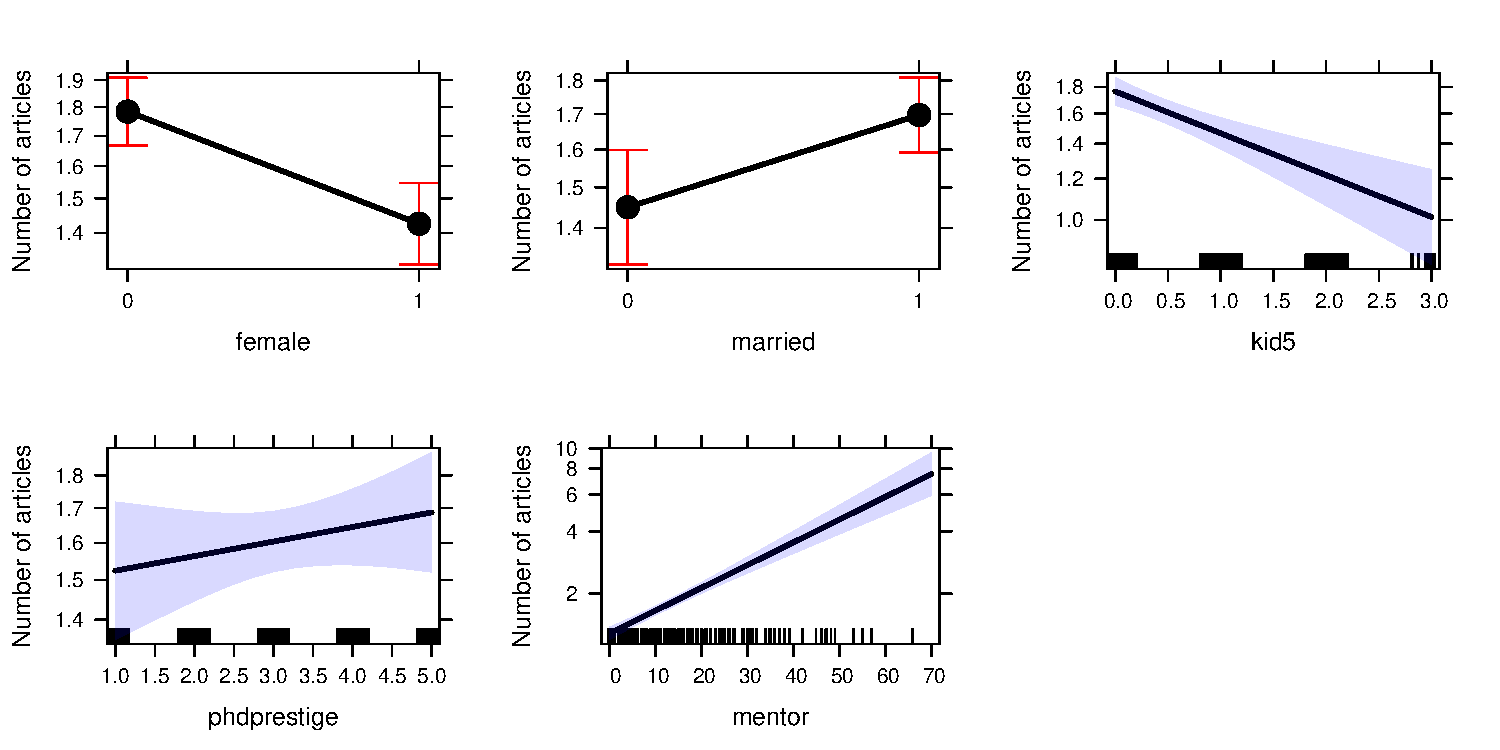
\includegraphics[width=\textwidth]{ch09/fig/phdpubs1-effpois} }

\caption[Effect plots for the predictors in the Poisson regression model for the PhdPubs data]{Effect plots for the predictors in the Poisson regression model for the PhdPubs data. Jittered values of the continuous predictors are shown at the bottom as rug-plots.\label{fig:phdpubs1-effpois}}
\end{figure}


\end{knitrout}

In \figref{fig:phdpubs1-effpois} we can see the decrease in published articles with
number of young children, but also that the confidence band gets wider with increasing
children.  The predicted effect here of number of publications by the student's mentor is more
dramatic, particularly for those whose mentor were truly prolific.

You should note that the panels for the predictors in \figref{fig:phdpubs1-effpois} are scaled
individually for the range of the fitted main effects.  This is often a sensible default
and all predictors except \code{mentor} give a similar range here.  To make all of these
plots strictly comparable, provide a \code{ylim} argument, giving the range of the
response on the log scale, as below (but not shown here).
\begin{knitrout}
\definecolor{shadecolor}{rgb}{1, 0.961, 0.933}\color{fgcolor}\begin{kframe}
\begin{alltt}
\hlkwd{plot}\hlstd{(}\hlkwd{allEffects}\hlstd{(phd.pois),} \hlkwc{band.colors}\hlstd{=}\hlstr{"blue"}\hlstd{,} \hlkwc{ylim}\hlstd{=}\hlkwd{c}\hlstd{(}\hlnum{0}\hlstd{,}\hlkwd{log}\hlstd{(}\hlnum{10}\hlstd{)))}
\end{alltt}
\end{kframe}
\end{knitrout}

All of the above is useful, but still leaves aside the question of how well the Poisson model fits
the data. The output from \code{summary(phd.pois)} above showed that the Poisson model fits quite badly.
The residual deviance of 1633.6 with 909 degrees
of freedom is highly significant.

\end{Example}



\begin{Example}[crabs1]{Mating of horseshoe crabs}
\citet{Brockmann:1996} studied the mating behavior of female horseshoe crabs in the Gulf of Mexico.
In the mating season, crabs arrive on the beach in female/male pairs to lay and fertilize eggs.
However, unattached males, called ``satellites,''
also come to the beach, crowd around the nesting couples and compete with attached males for fertilizations,
contributing to reproductive success.
Some females are ignored by satellite males, and some attract
more satellites than others, and the question is: what factors contribute to
to the number of satellites for each female? Or, perhaps better, how do unattached males choose among
available females?
This is another example in which zero counts
may require special treatment.

The data, given in \data{CrabSatellites} in the \Rpackage{countreg}, give the 
response variable, \code{satellites} for 173 females.  Possible predictors
are the female's \code{color} and \code{spine} condition, given as ordered factors,
as well as her \code{weight} and carapace (shell) \code{width}.

\begin{knitrout}\footnotesize
\definecolor{shadecolor}{rgb}{1, 0.961, 0.933}\color{fgcolor}\begin{kframe}
\begin{alltt}
\hlkwd{data}\hlstd{(}\hlstr{"CrabSatellites"}\hlstd{,} \hlkwc{package} \hlstd{=} \hlstr{"countreg"}\hlstd{)}
\hlkwd{str}\hlstd{(CrabSatellites)}
\end{alltt}
\begin{verbatim}
## 'data.frame':	173 obs. of  5 variables:
##  $ color     : Ord.factor w/ 4 levels "lightmedium"<..: 2 3 3 4 2 1 4 2 2 2 ...
##  $ spine     : Ord.factor w/ 3 levels "bothgood"<"onebroken"<..: 3 3 3 2 3 2 3 3 1 3 ...
##  $ width     : num  28.3 26 25.6 21 29 25 26.2 24.9 25.7 27.5 ...
##  $ weight    : num  3.05 2.6 2.15 1.85 3 2.3 1.3 2.1 2 3.15 ...
##  $ satellites: int  8 4 0 0 1 3 0 0 8 6 ...
\end{verbatim}
\end{kframe}
\end{knitrout}

\citet[\S 4.3]{Agresti:2013} analyses the number of satellites using count data
GLMs, and in his \C 5, describes separate logistic regression models for the binary
outcome of one or more satellites vs.\ none.  Later in this chapter (\secref{sec:glm-zeros})
we consider
hurdle and zero-inflated models for count data.  These have the advantage of 
modeling the zero counts together with a model for the positive counts.

A useful overview plot of the data is shown using \func{gpairs} in \figref{fig:crabs1-gpairs}.
You can see that the distribution of \var{satellites} is quite positively skewed,
with many zero counts.  \var{width} and \var{weight} are highly corrrelated (0.89),
and both relate to the size of the female.
Their scatterplots in the first row show that larger females attract more satellites.
The categorical ordered factors \var{spine} condition and \var{color} are strongly
associated, with the lightest colored crabs having the best conditions.
\begin{knitrout}
\definecolor{shadecolor}{rgb}{1, 0.961, 0.933}\color{fgcolor}\begin{kframe}
\begin{alltt}
\hlkwd{library}\hlstd{(vcd)}
\hlkwd{library}\hlstd{(gpairs)}
\hlkwd{gpairs}\hlstd{(CrabSatellites[,}\hlnum{5}\hlopt{:}\hlnum{1}\hlstd{],}
       \hlkwc{diag.pars} \hlstd{=} \hlkwd{list}\hlstd{(}\hlkwc{fontsize}\hlstd{=}\hlnum{16}\hlstd{),}
       \hlkwc{mosaic.pars} \hlstd{=} \hlkwd{list}\hlstd{(}\hlkwc{gp}\hlstd{=shading_Friendly,} \hlkwc{gp_args}\hlstd{=}\hlkwd{list}\hlstd{(}\hlkwc{interpolate}\hlstd{=}\hlnum{1}\hlopt{:}\hlnum{4}\hlstd{)))}
\end{alltt}
\end{kframe}\begin{figure}[!htbp]


\centerline{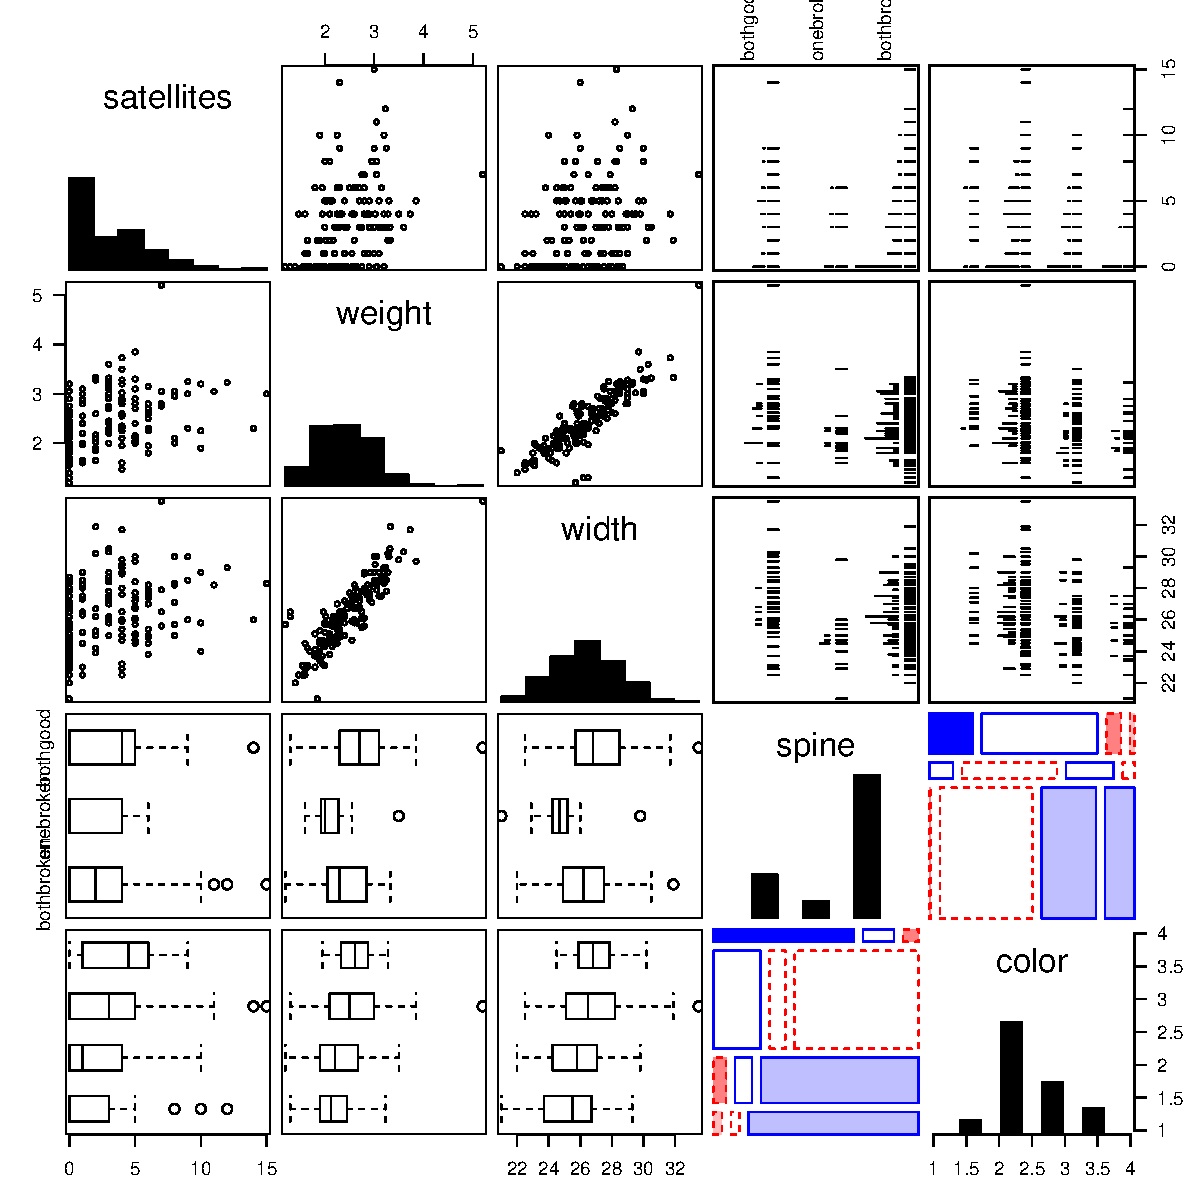
\includegraphics[width=.8\textwidth]{ch09/fig/crabs1-gpairs} }

\caption[Generalized pairs plot for the CrabSatellites data]{Generalized pairs plot for the CrabSatellites data.\label{fig:crabs1-gpairs}}
\end{figure}


\end{knitrout}

\figref{fig:crabs1-scats} shows the scatterplots of \var{satellites} against \var{width} and \var{weight}
together with smoothed lowess curves.  
\begin{knitrout}
\definecolor{shadecolor}{rgb}{1, 0.961, 0.933}\color{fgcolor}\begin{kframe}
\begin{alltt}
\hlkwd{plot}\hlstd{(}\hlkwd{jitter}\hlstd{(satellites)} \hlopt{~} \hlstd{width,} \hlkwc{data}\hlstd{=CrabSatellites,}
  \hlkwc{ylab}\hlstd{=}\hlstr{"Number of satellites (jittered)"}\hlstd{,} \hlkwc{xlab}\hlstd{=}\hlstr{"Carapace width"}\hlstd{,}
  \hlkwc{cex.lab}\hlstd{=}\hlnum{1.25}\hlstd{)}
\hlkwd{with}\hlstd{(CrabSatellites,} \hlkwd{lines}\hlstd{(}\hlkwd{lowess}\hlstd{(width, satellites),} \hlkwc{col}\hlstd{=}\hlstr{"red"}\hlstd{,} \hlkwc{lwd}\hlstd{=}\hlnum{2}\hlstd{))}
\hlkwd{plot}\hlstd{(}\hlkwd{jitter}\hlstd{(satellites)} \hlopt{~} \hlstd{weight,} \hlkwc{data}\hlstd{=CrabSatellites,}
  \hlkwc{ylab}\hlstd{=}\hlstr{"Number of satellites (jittered)"}\hlstd{,} \hlkwc{xlab}\hlstd{=}\hlstr{"Weight"}\hlstd{,}
  \hlkwc{cex.lab}\hlstd{=}\hlnum{1.25}\hlstd{)}
\hlkwd{with}\hlstd{(CrabSatellites,} \hlkwd{lines}\hlstd{(}\hlkwd{lowess}\hlstd{(weight, satellites),} \hlkwc{col}\hlstd{=}\hlstr{"red"}\hlstd{,} \hlkwc{lwd}\hlstd{=}\hlnum{2}\hlstd{))}
\end{alltt}
\end{kframe}\begin{figure}[!htbp]


\centerline{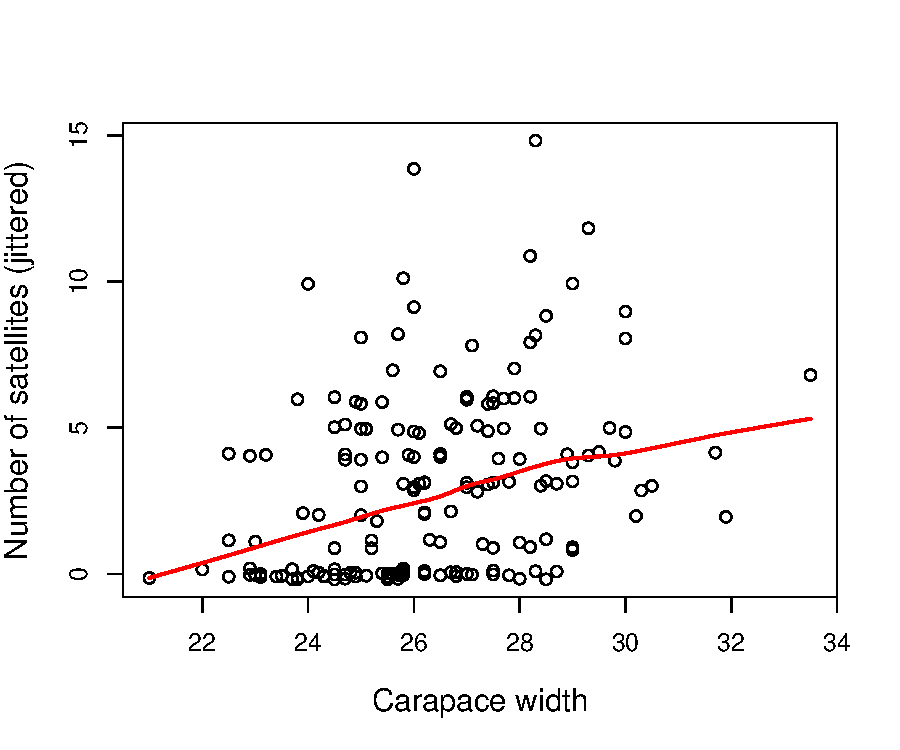
\includegraphics[width=.49\textwidth]{ch09/fig/crabs1-scats1} 
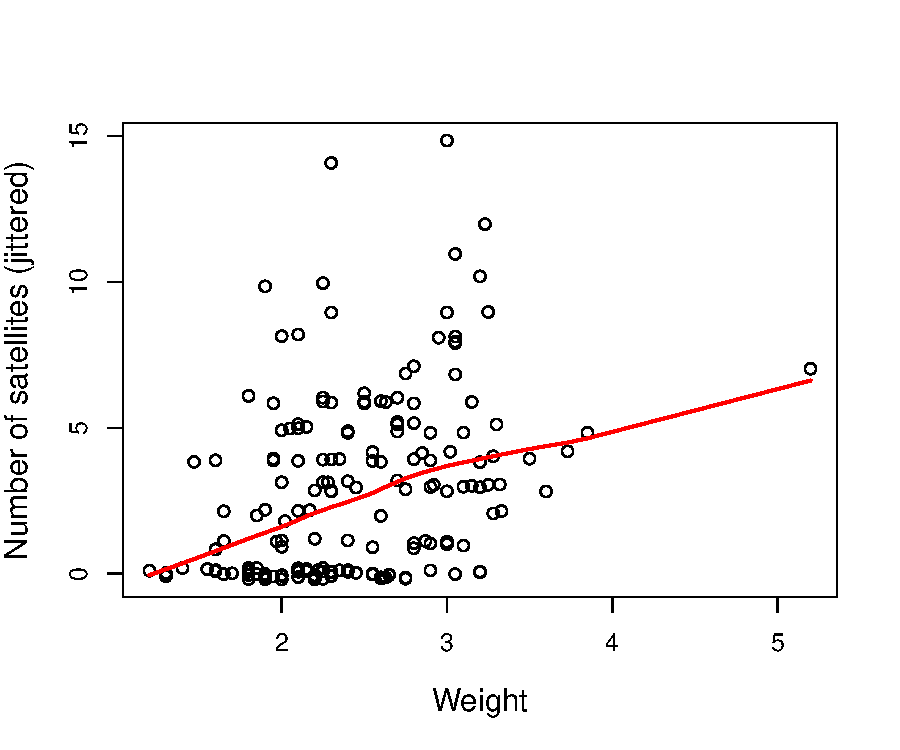
\includegraphics[width=.49\textwidth]{ch09/fig/crabs1-scats2} }

\caption[Scatterplots of number of satellites vs]{Scatterplots of number of satellites vs. width and weight, with lowess smooths.\label{fig:crabs1-scats}}
\end{figure}


\end{knitrout}
Both variables show approximately linear relations to the mean number of satellites, so it
would not be unreasonable to fit models using the identity link ($\mu \sim x$) rather than the log link
($\mu \sim \log(x)$) with the Poisson family GLM. 

In these plots, we reduce the problem of overplotting of the discrete response by jittering, but
an alternative technique is to transform a numeric count or continuous predictor to
a factor (for visualization purposes only), thereby giving boxplots.  A convenience function for
this purpose, \func{cutfac} is defined below.  It acts like \func{cut}, but gives nicer labels
for the factor levels and by default chooses convenient breaks among the values based on deciles.

\begin{knitrout}\footnotesize
\definecolor{shadecolor}{rgb}{1, 0.961, 0.933}\color{fgcolor}\begin{kframe}
\begin{alltt}
\hlstd{cutfac} \hlkwb{<-} \hlkwa{function}\hlstd{(}\hlkwc{x}\hlstd{,} \hlkwc{breaks} \hlstd{=} \hlkwa{NULL}\hlstd{,} \hlkwc{q}\hlstd{=}\hlnum{10}\hlstd{) \{}
  \hlkwa{if}\hlstd{(}\hlkwd{is.null}\hlstd{(breaks)) breaks} \hlkwb{<-} \hlkwd{unique}\hlstd{(}\hlkwd{quantile}\hlstd{(x,} \hlnum{0}\hlopt{:}\hlstd{q}\hlopt{/}\hlstd{q))}
  \hlstd{x} \hlkwb{<-} \hlkwd{cut}\hlstd{(x, breaks,} \hlkwc{include.lowest} \hlstd{=} \hlnum{TRUE}\hlstd{,} \hlkwc{right} \hlstd{=} \hlnum{FALSE}\hlstd{)}
  \hlkwd{levels}\hlstd{(x)} \hlkwb{<-} \hlkwd{paste}\hlstd{(breaks[}\hlopt{-}\hlkwd{length}\hlstd{(breaks)],} \hlkwd{ifelse}\hlstd{(}\hlkwd{diff}\hlstd{(breaks)} \hlopt{>} \hlnum{1}\hlstd{,}
    \hlkwd{c}\hlstd{(}\hlkwd{paste}\hlstd{(}\hlstr{"-"}\hlstd{, breaks[}\hlopt{-}\hlkwd{c}\hlstd{(}\hlnum{1}\hlstd{,} \hlkwd{length}\hlstd{(breaks))]} \hlopt{-} \hlnum{1}\hlstd{,} \hlkwc{sep} \hlstd{=} \hlstr{""}\hlstd{),} \hlstr{"+"}\hlstd{),} \hlstr{""}\hlstd{),} \hlkwc{sep} \hlstd{=} \hlstr{""}\hlstd{)}
  \hlkwd{return}\hlstd{(x)}
\hlstd{\}}
\end{alltt}
\end{kframe}
\end{knitrout}

Using this, the plots in \figref{fig:crabs1-scats} can be re-drawn as boxplots, giving \figref{fig:crabs1-boxplots}.

\begin{knitrout}
\definecolor{shadecolor}{rgb}{1, 0.961, 0.933}\color{fgcolor}\begin{kframe}
\begin{alltt}
\hlkwd{plot}\hlstd{(satellites} \hlopt{~} \hlkwd{cutfac}\hlstd{(width),} \hlkwc{data}\hlstd{=CrabSatellites,}
     \hlkwc{ylab}\hlstd{=}\hlstr{"Number of satellites"}\hlstd{,} \hlkwc{xlab}\hlstd{=}\hlstr{"Carapace width (deciles)"}\hlstd{)}
\hlkwd{plot}\hlstd{(satellites} \hlopt{~} \hlkwd{cutfac}\hlstd{(weight),} \hlkwc{data}\hlstd{=CrabSatellites,}
     \hlkwc{ylab}\hlstd{=}\hlstr{"Number of satellites"}\hlstd{,} \hlkwc{xlab}\hlstd{=}\hlstr{"Weight (deciles)"}\hlstd{)}
\end{alltt}
\end{kframe}\begin{figure}[!htbp]


\centerline{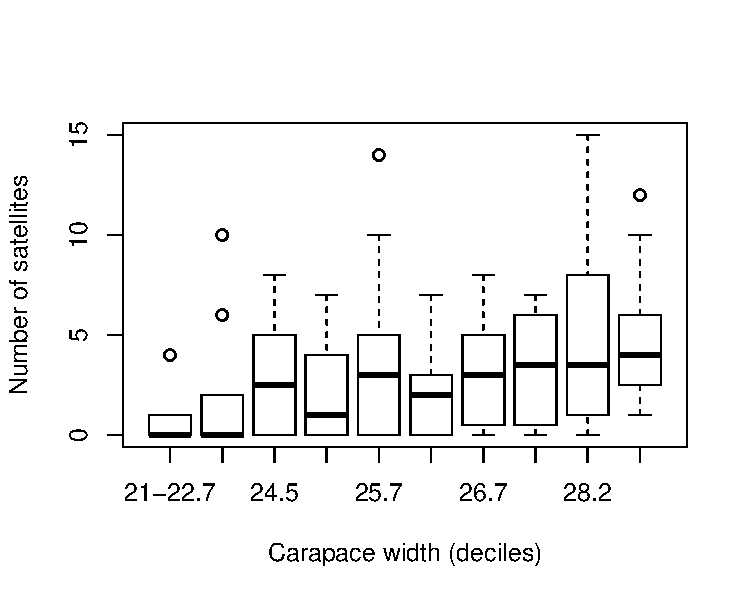
\includegraphics[width=.49\textwidth]{ch09/fig/crabs1-boxplots1} 
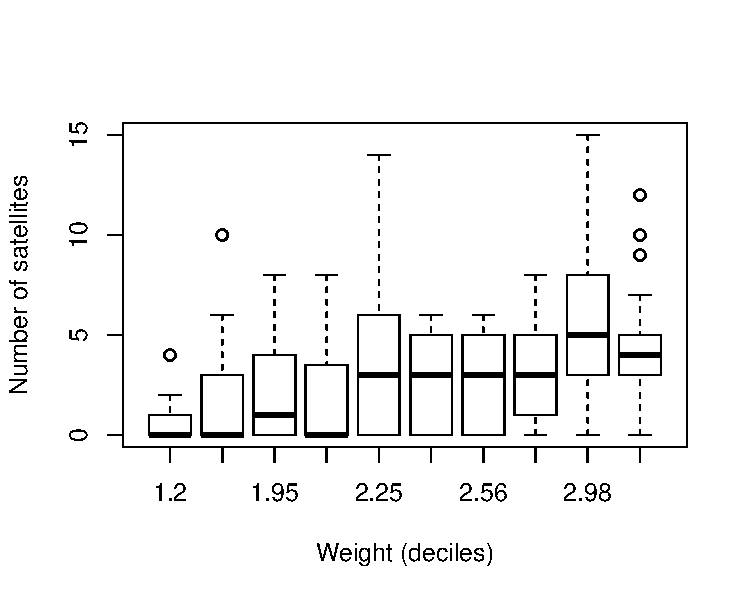
\includegraphics[width=.49\textwidth]{ch09/fig/crabs1-boxplots2} }

\caption[Boxplots of number of satellites vs]{Boxplots of number of satellites vs. width and weight.\label{fig:crabs1-boxplots}}
\end{figure}


\end{knitrout}

Wih this visual overview, we proceed to an initial Poisson GLM model, using all predictors.
Note that \var{color} and \var{spine} are ordered factors, so \func{glm} represents them
as polynomial contrasts, as if they were coded numerically.

\begin{knitrout}
\definecolor{shadecolor}{rgb}{1, 0.961, 0.933}\color{fgcolor}\begin{kframe}
\begin{alltt}
\hlstd{crabs.pois} \hlkwb{<-} \hlkwd{glm}\hlstd{(satellites} \hlopt{~} \hlstd{.,} \hlkwc{data}\hlstd{=CrabSatellites,} \hlkwc{family}\hlstd{=poisson)}
\hlkwd{summary}\hlstd{(crabs.pois)}
\end{alltt}
\begin{verbatim}
...
## Coefficients:
##             Estimate Std. Error z value Pr(>|z|)   
## (Intercept)  -0.7057     0.9344   -0.76   0.4501   
## color.L      -0.4120     0.1567   -2.63   0.0085 **
## color.Q       0.1237     0.1231    1.00   0.3150   
## color.C       0.0481     0.0914    0.53   0.5983   
## spine.L       0.0618     0.0848    0.73   0.4660   
## spine.Q       0.1585     0.1609    0.99   0.3244   
## width         0.0165     0.0489    0.34   0.7358   
## weight        0.4971     0.1663    2.99   0.0028 **
## ---
## Signif. codes:  0 '***' 0.001 '**' 0.01 '*' 0.05 '.' 0.1 ' ' 1
## 
## (Dispersion parameter for poisson family taken to be 1)
## 
##     Null deviance: 632.79  on 172  degrees of freedom
## Residual deviance: 549.56  on 165  degrees of freedom
## AIC: 920.9
...
\end{verbatim}
\end{kframe}
\end{knitrout}
The Wald tests for the coefficients show that only the linear effect of color and the effect
of width are significant.  
Effect plots, in \figref{fig:crabs1-eff1}, show the nature of these
effects--- lighter colored females attact more satellites, as do wider and heavier females.

\begin{knitrout}
\definecolor{shadecolor}{rgb}{1, 0.961, 0.933}\color{fgcolor}\begin{kframe}
\begin{alltt}
\hlkwd{plot}\hlstd{(}\hlkwd{allEffects}\hlstd{(crabs.pois),} \hlkwc{main}\hlstd{=}\hlstr{""}\hlstd{)}
\end{alltt}
\end{kframe}\begin{figure}[!htbp]


\centerline{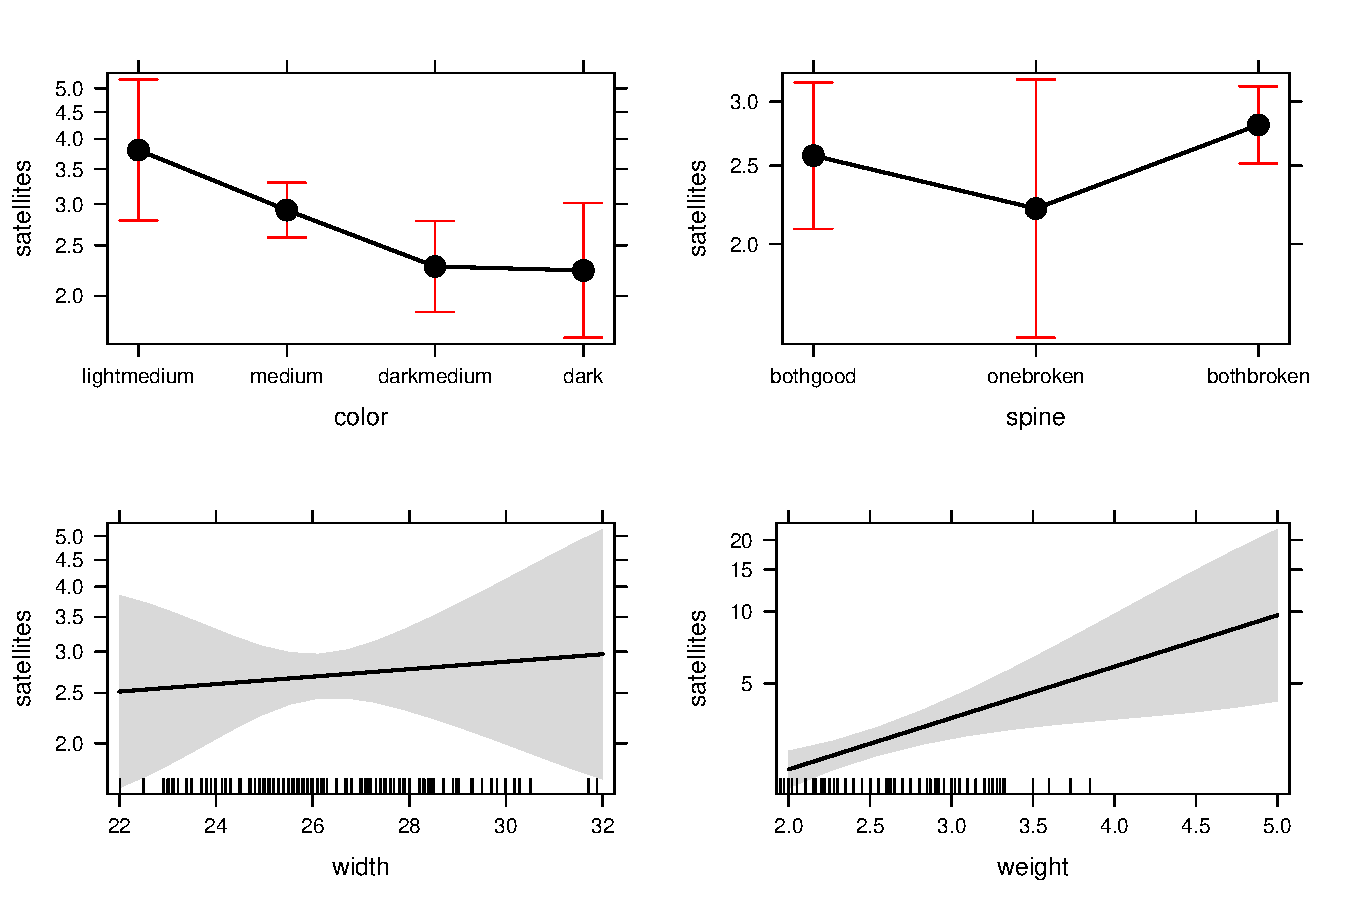
\includegraphics[width=\textwidth]{ch09/fig/crabs1-eff1} }

\caption[Effect plots for the predictors in the Poisson regression model for the CrabSatellites data]{Effect plots for the predictors in the Poisson regression model for the CrabSatellites data.\label{fig:crabs1-eff1}}
\end{figure}


\end{knitrout}

A simpler model can be constructed using \var{color} as a numeric variable, and either width or
weight to represent female size. We choose weight here.%
\footnote{
\citet[\S 4.3]{Agresti:2013} and others who have analyzed this example uses carapace width
as the main quantitative predictor, possibly because width might be more biologically salient
to the single males than weight.  This is a case where two 
highly correlated predictors are each strongly related to the outcome, 
yet partial tests (controlling for all others) may prefer one over the other.
}

\begin{knitrout}
\definecolor{shadecolor}{rgb}{1, 0.961, 0.933}\color{fgcolor}\begin{kframe}
\begin{alltt}
\hlstd{CrabSatellites1} \hlkwb{<-} \hlkwd{transform}\hlstd{(CrabSatellites,}
  \hlkwc{color} \hlstd{=} \hlkwd{as.numeric}\hlstd{(color))}

\hlstd{crabs.pois1} \hlkwb{<-} \hlkwd{glm}\hlstd{(satellites} \hlopt{~} \hlstd{weight} \hlopt{+} \hlstd{color,} \hlkwc{data}\hlstd{=CrabSatellites1,}
                   \hlkwc{family}\hlstd{=poisson)}
\hlkwd{summary}\hlstd{(crabs.pois1)}
\end{alltt}
\begin{verbatim}
...
## 
## Coefficients:
##             Estimate Std. Error z value Pr(>|z|)    
## (Intercept)   0.0888     0.2544    0.35    0.727    
## weight        0.5458     0.0675    8.09    6e-16 ***
## color        -0.1728     0.0615   -2.81    0.005 ** 
## ---
## Signif. codes:  0 '***' 0.001 '**' 0.01 '*' 0.05 '.' 0.1 ' ' 1
## 
## (Dispersion parameter for poisson family taken to be 1)
## 
##     Null deviance: 632.79  on 172  degrees of freedom
## Residual deviance: 552.77  on 170  degrees of freedom
## AIC: 914.1
...
\end{verbatim}
\end{kframe}
\end{knitrout}

From the statistical and graphical analysis so far, the answser to the question posed 
in this example is clear:  unattached male horseshoe crabs prefer light-colored
big, fat mamas!

Yet, neither of these models fit well, as can be seen from their residual deviances
and \LR tests.
\begin{knitrout}
\definecolor{shadecolor}{rgb}{1, 0.961, 0.933}\color{fgcolor}\begin{kframe}
\begin{alltt}
\hlstd{vcdExtra::}\hlkwd{Summarise}\hlstd{(crabs.pois, crabs.pois1)}
\end{alltt}
\begin{verbatim}
## Likelihood summary table:
##             AIC BIC LR Chisq Df Pr(>Chisq)    
## crabs.pois  921 946      550  8     <2e-16 ***
## crabs.pois1 914 924      553  3     <2e-16 ***
## ---
## Signif. codes:  0 '***' 0.001 '**' 0.01 '*' 0.05 '.' 0.1 ' ' 1
\end{verbatim}
\end{kframe}
\end{knitrout}
Perhaps there is something else to be learned here.

\end{Example}

\section{Models for overdispersed count data}\label{sec:glm-overdisp}

In practice, the Poisson model is often very useful for describing the
relationship between the mean $\mu_i$ and the linear predictors, 
but typically underestimates the variance in the data.
The consequence is that the Poisson standard errors are too small,
rendering the Wald tests of coefficients, $z_j = \widehat{\beta}_j / se(\widehat{\beta}_j) $
(and other hypothesis test statistics)
too large, and thus overly liberal.  

In applications of the GLM, overdispersion is usually assessed by the \LR
test of the deviance (or the Pearson statistic) given in \secref{sec:glm-goodfit},
but there is a subtle problem here. Lack of fit in a GLM for count data can result 
either from a mis-specified model for the systematic component
(omitted or unmeasured predictors, non-linear relations, etc.)
or from failure of the Poisson mean = variance assumption.
Thus, use of these methods requires some high degree of confidence that the
systematic part of the model has been correctly specified, so that any
lack of fit can be attributed to overdispersion.

One way of dealing with this is to base inference on 
so-called \emph{sandwich} covariance estimators that are robust against
some types of model mis-specification.  In \R, this is provided by the
\func{sandwich} function in the \Rpackage{sandwich}, and can be used
with \code{coeftest(model, vcov=sandwich)} to give overdispersion-corrected
hypothesis tests.
Alternatively, the Poisson model variance assumption can be relaxed
in the quasi-Poisson model and the negative-binomial model as
discussed below.
 

\subsection{The quasi-Poisson model}\label{sec:glm-quasi}

One obvious solution to the problem of overdispersion for count data is the relaxed assumption
that the conditional variance is merely \emph{proportional} to the mean,
\begin{equation*}
\V (y_i | \eta_i) = \phi \mu_i
\end{equation*}
Overdispersion is the common case of $\phi > 1$, implying that the conditional variance
increases faster than the mean, but the opposite case of underdispersion, $\phi < 1$
is also possible, though relatively rare in practice.
This strategy entails estimating the dispersion parameter $\phi$ from the data,
and gives the \term{quasi-Poisson model} for count data.

One possible estimate is the residual deviance divided by degrees of freedom.
However, it is more common to use the Pearson statistics, that gives
a method-of-moments estimate with improved statistical properties.
\begin{equation*}
\widehat{\phi} = 
\frac{X^2_P}{n-p} = 
\sum_{i=1}^n \frac{(y_i - \widehat{\mu}_i)^2}{\widehat{\mu}_i} \left/ (n-p) \right.
\end{equation*}

It turns out that this model gives the same coefficient estimates as the standard
Poisson GLM, but inference is adjusted for over/under dispersion.
In particular, following \eqref{eq:varbeta}
the standard errors of the model coefficients are multiplied by 
$\widehat{\phi}^{1/2}$ and so are inflated when overdispersion is present.
In \R, the quasi-Poisson model with this estimated dispersion parameter is
fitted with the \func{glm} function, by setting \code{family=quasipoisson}.

\begin{Example}[phdpubs2]{Publications of PhD candidates}

For the \data{PhdPubs} data, the deviance and Pearson estimates of dispersion $\phi$
can be calculated using the results of the Poisson model saved in the
\code{phd.pois} object.  The Pearson estimate, 1.83, indicates that
standard errors of coefficients in this model should be multiplied by
$\sqrt{1.83} = 1.35$, a 35\% increase, to correct for overdispersion.

\begin{knitrout}
\definecolor{shadecolor}{rgb}{1, 0.961, 0.933}\color{fgcolor}\begin{kframe}
\begin{alltt}
\hlkwd{with}\hlstd{(phd.pois, deviance}\hlopt{/}\hlstd{df.residual)}
\end{alltt}
\begin{verbatim}
## [1] 1.797
\end{verbatim}
\begin{alltt}
\hlkwd{sum}\hlstd{(}\hlkwd{residuals}\hlstd{(phd.pois,} \hlkwc{type} \hlstd{=} \hlstr{"pearson"}\hlstd{)}\hlopt{^}\hlnum{2}\hlstd{)}\hlopt{/}\hlstd{phd.pois}\hlopt{$}\hlstd{df.residual}
\end{alltt}
\begin{verbatim}
## [1] 1.83
\end{verbatim}
\end{kframe}
\end{knitrout}
The quasi-Poisson model is then fitted using \func{glm} as:
\begin{knitrout}
\definecolor{shadecolor}{rgb}{1, 0.961, 0.933}\color{fgcolor}\begin{kframe}
\begin{alltt}
\hlstd{phd.qpois} \hlkwb{<-} \hlkwd{glm}\hlstd{(articles} \hlopt{~} \hlstd{.,} \hlkwc{data}\hlstd{=PhdPubs,} \hlkwc{family}\hlstd{=quasipoisson)}
\end{alltt}
\end{kframe}
\end{knitrout}
For use in other computation, the  dispersion parameter estimate $\widehat{\phi}$ can be obtained as the 
\code{dispersion} value of the \func{summary} method for a quasi-Poisson model.
\begin{knitrout}
\definecolor{shadecolor}{rgb}{1, 0.961, 0.933}\color{fgcolor}\begin{kframe}
\begin{alltt}
\hlstd{(phi} \hlkwb{<-} \hlkwd{summary}\hlstd{(phd.qpois)}\hlopt{$}\hlstd{dispersion)}
\end{alltt}
\begin{verbatim}
## [1] 1.83
\end{verbatim}
\end{kframe}
\end{knitrout}
Note that this value can be compared to the variance/mean ratio of 2.91 calculated for the 
marginal distribution in \exref{ex:phdpubs1}; there is considerable improvement taking the
predictors into account.

\end{Example}

\subsection{The negative-binomial model}\label{sec:glm-negbin}

The negative-biomial model for count data was introduced in \secref{sec:negbin}
as a different generalization of the Poisson model that allows for overdispersion. 
In the context of the GLM, this can be developed as the extended form where
the distribution of $y_i \given \vec{x}_i$ where the mean $\mu_i$ for fixed
$\vec{x}_i$ can vary across observations $i$ according to a gamma distribution 
with mean $\mu_i$ and a constant shape parameter, $\theta$, reflecting the
additional variation due to heterogeneity.

For a fixed value of $\theta$, the negative-binomial is another special case of
the GLM.
The expected value of the response is again
$\E(y_i) = \mu_i$, but the variance function is $\V(y_i) = \mu_i + \mu_i^2 / \theta$,
so the variance of $y$ increases more rapidly than that of the Poisson distribution.
Some authors (e.g., \citet{Agresti:2013,Hilbe:2014}) prefer to parameterize the variance
function in terms of $\alpha = 1/\theta$, giving
\begin{equation*}
\V(y_i) = \mu_i + \mu_i^2 / \theta = \mu_i + \alpha \mu_i^2 \comma
\end{equation*}
so that $\alpha$ is a kind of dispersion parameter.  Note that as $\alpha \rightarrow 0$,
$\V(y_i) \rightarrow \mu_i$ and the negative-binomial converges to the Poisson.

The \Rpackage{MASS} provides the family function \code{negative.binomial(theta)} that
can be used directly with \func{glm} provided that the argument \code{theta} is specified.
One example would be the related geometric distribution (\secref{sec:geometric}),
that is the special case of $\theta=1$. This can be fitted in \R by setting
\code{family=negative.binomial(theta=1)} in the call to \func{glm}.

Most often, $\theta$ is unknown and must be estimated from the data.
In this case, the negative-binomial model is not a special case of the GLM, 
but it is possible to obtain maximum likelihood estimates of both
$\vec{\beta}$ and $\theta$, by iteratively estimating $\vec{\beta}$ for fixed $\theta$
and vice-versa. This method is implemented in the \func{glm.nb} in the package \pkg{MASS}.

\begin{Example}[crabs-nbin]{Mating of horseshoe crabs}
For example, for the \data{CrabSatellites} data,
we can fit the general negative-binomial model with
$\theta$ free.
\begin{knitrout}
\definecolor{shadecolor}{rgb}{1, 0.961, 0.933}\color{fgcolor}\begin{kframe}
\begin{alltt}
\hlkwd{library}\hlstd{(MASS)}
\hlstd{crabs.nbin} \hlkwb{<-} \hlkwd{glm.nb}\hlstd{(satellites} \hlopt{~} \hlstd{weight} \hlopt{+} \hlstd{color,} \hlkwc{data}\hlstd{=CrabSatellites1)}
\hlstd{crabs.nbin}\hlopt{$}\hlstd{theta}
\end{alltt}
\begin{verbatim}
## [1] 0.9556
\end{verbatim}
\end{kframe}
\end{knitrout}
The estimated value $\widehat{\theta}$ returned by \func{glm.nb} is not very far from 1.
Hence, we might also consider fixing $\theta=1$, as illustrated below.
\begin{knitrout}
\definecolor{shadecolor}{rgb}{1, 0.961, 0.933}\color{fgcolor}\begin{kframe}
\begin{alltt}
\hlstd{crabs.nbin1} \hlkwb{<-} \hlkwd{glm}\hlstd{(satellites} \hlopt{~} \hlstd{weight} \hlopt{+} \hlstd{color,} \hlkwc{data}\hlstd{=CrabSatellites1,}
                   \hlkwc{family}\hlstd{=}\hlkwd{negative.binomial}\hlstd{(}\hlnum{1}\hlstd{))}
\end{alltt}
\end{kframe}
\end{knitrout}
\end{Example}

% until I finish the negbin section....



\subsection{Visualizing the mean--variance relation}

The quasi-Poisson and negative-binomial models have different variance functions, and one way to
visualize which provides a better fit to the data is to group the data according to the
fitted value of the linear predictor, calculate the mean and variance for each group, and
then plot the variances against the means.
A smoothed curve will then approximate the \emph{empirical} mean--variance relationship.
To this, we can add curves showing the mean--variance function implied by various models.%
\footnote{
This idea and the example that follows was suggested by Germ\'an Rodrigues
in a Stata example given at
\url{http://data.princeton.edu/wws509/stata/overdispersion.html}.
}

\begin{Example}[phdpubs3]{Publications of PhD candidates}
For the \data{PhdPubs} data, the fitted values are obtained with \func{fitted} for the
Poisson and negative binomial models. Either set can be used to categorize the observations
into groups for the purpose of calculating means and variances of the response.


\begin{knitrout}
\definecolor{shadecolor}{rgb}{1, 0.961, 0.933}\color{fgcolor}\begin{kframe}
\begin{alltt}
\hlstd{fit.pois} \hlkwb{<-} \hlkwd{fitted}\hlstd{(phd.pois,} \hlkwc{type}\hlstd{=}\hlstr{"response"}\hlstd{)}
\hlstd{fit.nbin} \hlkwb{<-} \hlkwd{fitted}\hlstd{(phd.nbin,} \hlkwc{type}\hlstd{=}\hlstr{"response"}\hlstd{)}
\end{alltt}
\end{kframe}
\end{knitrout}
Here we use a simpler version of the \func{cutfac} function to group a numeric variable
into quantile-based groups.  \func{cutq} also uses deciles by default, and just uses
simple integer values for the factor labels.
\begin{knitrout}
\definecolor{shadecolor}{rgb}{1, 0.961, 0.933}\color{fgcolor}\begin{kframe}
\begin{alltt}
\hlstd{cutq} \hlkwb{<-} \hlkwa{function}\hlstd{(}\hlkwc{x}\hlstd{,} \hlkwc{q} \hlstd{=} \hlnum{10}\hlstd{) \{}
    \hlstd{quantile} \hlkwb{<-} \hlkwd{cut}\hlstd{(x,} \hlkwc{breaks} \hlstd{=} \hlkwd{quantile}\hlstd{(x,} \hlkwc{probs} \hlstd{=} \hlnum{0}\hlopt{:}\hlstd{q}\hlopt{/}\hlstd{q),}
        \hlkwc{include.lowest} \hlstd{=} \hlnum{TRUE}\hlstd{,} \hlkwc{labels} \hlstd{=} \hlnum{1}\hlopt{:}\hlstd{q)}
    \hlstd{quantile}
\hlstd{\}}
\end{alltt}
\end{kframe}
\end{knitrout}
Using this, we create a variable \code{group} giving 20 quantile groups of the fitted values,
and then use \func{aggregate} to find the mean and variance of the number of articles
in each group.
\begin{knitrout}
\definecolor{shadecolor}{rgb}{1, 0.961, 0.933}\color{fgcolor}\begin{kframe}
\begin{alltt}
\hlstd{group} \hlkwb{<-} \hlkwd{cutq}\hlstd{(fit.nbin,} \hlkwc{q}\hlstd{=}\hlnum{20}\hlstd{)}
\hlstd{qdat} \hlkwb{<-} \hlkwd{aggregate}\hlstd{(PhdPubs}\hlopt{$}\hlstd{articles,}
          \hlkwd{list}\hlstd{(group),}
          \hlkwc{FUN} \hlstd{=} \hlkwa{function}\hlstd{(}\hlkwc{x}\hlstd{)} \hlkwd{c}\hlstd{(}\hlkwc{mean}\hlstd{=}\hlkwd{mean}\hlstd{(x),} \hlkwc{var}\hlstd{=}\hlkwd{var}\hlstd{(x)))}
\hlstd{qdat} \hlkwb{<-} \hlkwd{data.frame}\hlstd{(qdat}\hlopt{$}\hlstd{x)}
\hlstd{qdat} \hlkwb{<-} \hlstd{qdat[}\hlkwd{order}\hlstd{(qdat}\hlopt{$}\hlstd{mean),]}
\end{alltt}
\end{kframe}
\end{knitrout}
We can then calculate the theoretical variances implied by the quasi-Poisson and negative-binomial models:
\begin{knitrout}
\definecolor{shadecolor}{rgb}{1, 0.961, 0.933}\color{fgcolor}\begin{kframe}
\begin{alltt}
\hlstd{phi} \hlkwb{<-} \hlkwd{summary}\hlstd{(phd.qpois)}\hlopt{$}\hlstd{dispersion}
\hlstd{qdat}\hlopt{$}\hlstd{qvar} \hlkwb{<-} \hlstd{phi} \hlopt{*} \hlstd{qdat}\hlopt{$}\hlstd{mean}
\hlstd{qdat}\hlopt{$}\hlstd{nbvar} \hlkwb{<-} \hlstd{qdat}\hlopt{$}\hlstd{mean} \hlopt{+} \hlstd{(qdat}\hlopt{$}\hlstd{mean}\hlopt{^}\hlnum{2}\hlstd{)} \hlopt{/} \hlstd{phd.nbin}\hlopt{$}\hlstd{theta}
\hlkwd{head}\hlstd{(qdat)}
\end{alltt}
\begin{verbatim}
##     mean   var  qvar  nbvar
## 1 0.6122 0.784 1.121 0.7776
## 2 1.1489 1.782 2.103 1.7312
## 8 1.2444 2.462 2.278 1.9276
## 4 1.2609 1.708 2.308 1.9622
## 6 1.2727 1.831 2.330 1.9873
## 7 1.2979 4.344 2.376 2.0409
\end{verbatim}
\end{kframe}
\end{knitrout}
The plot, shown in \figref{fig:phd-mean-var-plot}, then simply plots the points and
uses \func{lines} to plot the model-implied variances.
\begin{knitrout}
\definecolor{shadecolor}{rgb}{1, 0.961, 0.933}\color{fgcolor}\begin{kframe}
\begin{alltt}
\hlkwd{with}\hlstd{(qdat, \{}
  \hlkwd{plot}\hlstd{(var} \hlopt{~} \hlstd{mean,} \hlkwc{xlab}\hlstd{=}\hlstr{"Mean number of articles"}\hlstd{,} \hlkwc{ylab}\hlstd{=}\hlstr{"Variance"}\hlstd{,}
       \hlkwc{pch}\hlstd{=}\hlnum{16}\hlstd{,} \hlkwc{cex}\hlstd{=}\hlnum{1.2}\hlstd{,} \hlkwc{cex.lab}\hlstd{=}\hlnum{1.2}\hlstd{)}
  \hlkwd{abline}\hlstd{(}\hlkwc{h}\hlstd{=}\hlkwd{mean}\hlstd{(PhdPubs}\hlopt{$}\hlstd{articles),} \hlkwc{col}\hlstd{=}\hlkwd{gray}\hlstd{(}\hlnum{.40}\hlstd{),} \hlkwc{lty}\hlstd{=}\hlstr{"dotted"}\hlstd{)}
  \hlkwd{lines}\hlstd{(mean, qvar,} \hlkwc{col}\hlstd{=}\hlstr{"red"}\hlstd{,} \hlkwc{lwd}\hlstd{=}\hlnum{2}\hlstd{)}
  \hlkwd{lines}\hlstd{(mean, nbvar,} \hlkwc{col}\hlstd{=}\hlstr{"blue"}\hlstd{,} \hlkwc{lwd}\hlstd{=}\hlnum{2}\hlstd{)}
  \hlkwd{lines}\hlstd{(}\hlkwd{lowess}\hlstd{(mean, var),} \hlkwc{lwd}\hlstd{=}\hlnum{2}\hlstd{,} \hlkwc{lty}\hlstd{=}\hlstr{"dashed"}\hlstd{)}
  \hlkwd{text}\hlstd{(}\hlnum{3}\hlstd{,} \hlkwd{mean}\hlstd{(PhdPubs}\hlopt{$}\hlstd{articles),} \hlstr{"Poisson"}\hlstd{,} \hlkwc{col}\hlstd{=}\hlkwd{gray}\hlstd{(}\hlnum{.40}\hlstd{))}
  \hlkwd{text}\hlstd{(}\hlnum{3}\hlstd{,} \hlnum{5}\hlstd{,} \hlstr{"quasi-Poisson"}\hlstd{,} \hlkwc{col}\hlstd{=}\hlstr{"red"}\hlstd{)}
  \hlkwd{text}\hlstd{(}\hlnum{3}\hlstd{,} \hlnum{6.7}\hlstd{,} \hlstr{"negbin"}\hlstd{,} \hlkwc{col}\hlstd{=}\hlstr{"blue"}\hlstd{)}
  \hlkwd{text}\hlstd{(}\hlnum{3}\hlstd{,} \hlnum{8.5}\hlstd{,} \hlstr{"lowess"}\hlstd{)}
\hlstd{\})}
\end{alltt}
\end{kframe}\begin{figure}[!htbp]


\centerline{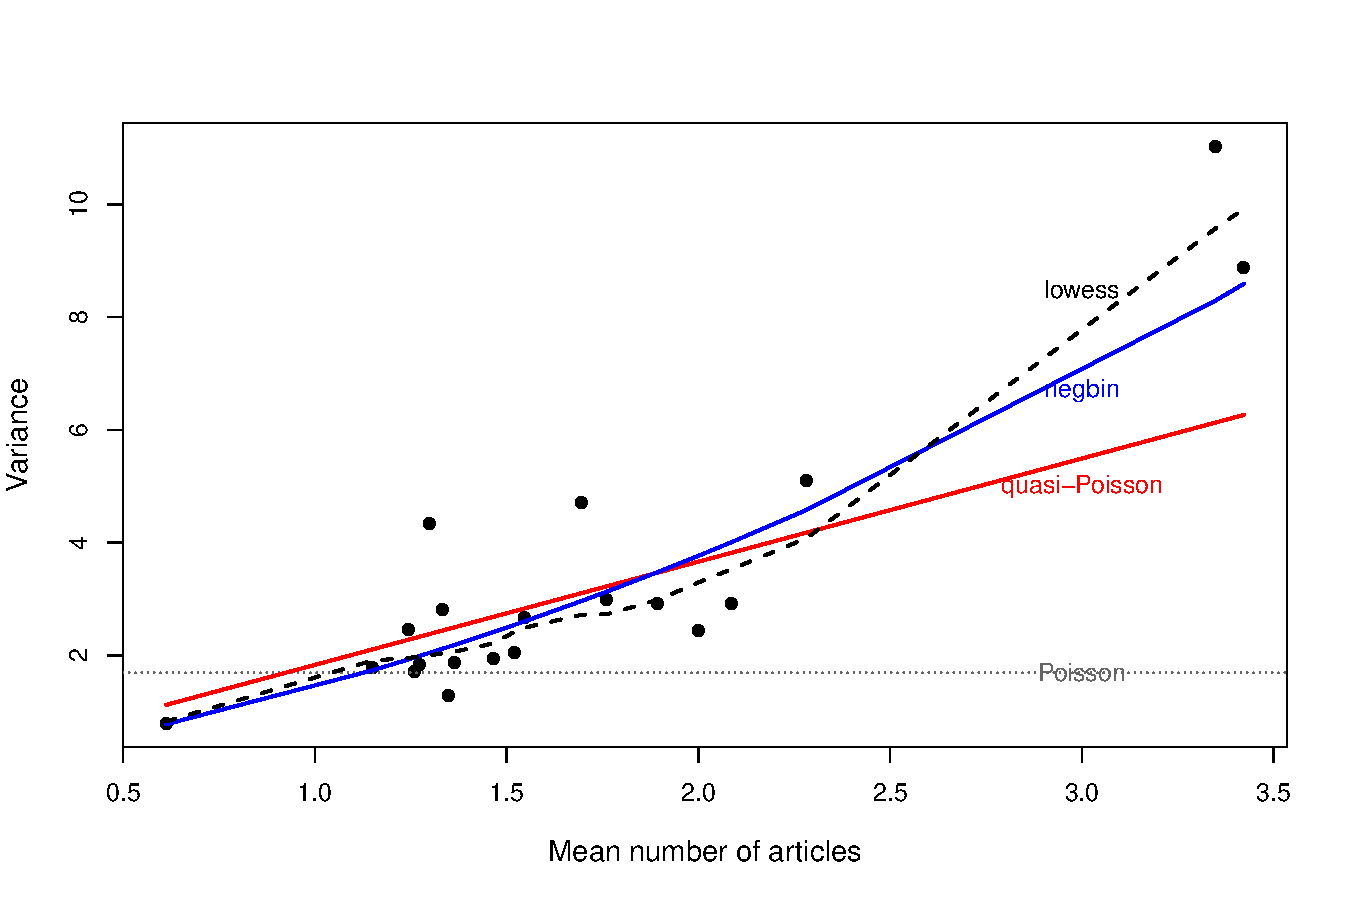
\includegraphics[width=.75\textwidth]{ch09/fig/phd-mean-var-plot} }

\caption[Mean--variance functions for the PhdPubs data]{Mean--variance functions for the PhdPubs data. Points show the observed means and variances for 20 quantile groups based on the fitted values in the negative-binomial model. The labeled lines and curves show the variance functions implied by various models.\label{fig:phd-mean-var-plot}}
\end{figure}


\end{knitrout}
We can see from this plot that the variances implied by the quasi-Poisson and negative-binomial
models are in reasonable accord with the data and with each other up to a mean of about 2.5.
They diverge substantially at the upper end, for the 20--30\% of the most productive
candidates, where the quadratic variance function of the negative-binomial provides a
better fit.

\end{Example}

\subsection{Visualizing goodness-of-fit}\label{sec:glm-visfit}

Even with correction for overdispersion, goodness-of-fit tests provide only an overall
summary of model fit.  Some specialized tests for particular forms of overdispersion
are also available (e.g., see \citet[\C 5]{CameronTrivedi:1998}),
but these only identify general problems and cannot provide detailed indications of
the possible source of these problems.

In \chref{ch:discrete}, we illustrated the use of rootograms for visualizing goodness-of-fit
to a wide variety discrete distributions using the \func{plot} method for
class \class{goodfit} objects with the \Rpackage{vcd}.  However, those methods were
developed for one-way discrete distributions without explanatory variables.

\citet{KleiberZeileis:2014} have generalized this idea to the wider class of 
GLM-related count regression models considered here.
The \Rpackage{countreg} provides a new implementation of \func{rootogram}
with methods for all of these models (and others not metioned).
We illustrate these plots for the models considered to this point, and then extend
this use for models allowing for excess zero counts in \secref{sec:glm-zeros}.

\begin{Example}[phdpubs4]{Publications of PhD candidates}
For the \data{PhdPubs} data, \figref{fig:phdpubs4-rootogram} shows hanging rootograms for the
Poisson and negative-binomial models produced using \code{countreg::rootogram}%
\footnote{
At the time of this writing, \code{rootogram} in \pkg{countreg} conflicts with
the version in \pkg{vcd}, so we qualify the use here with the package name.
}
on the fitted model objects.  We are looking both for general patterns of under/over fit, as well
as counts that stand out as poorly fitted against the background.

\begin{knitrout}
\definecolor{shadecolor}{rgb}{1, 0.961, 0.933}\color{fgcolor}\begin{kframe}
\begin{alltt}
\hlkwd{library}\hlstd{(countreg)}
\hlstd{countreg::}\hlkwd{rootogram}\hlstd{(phd.pois,} \hlkwc{max}\hlstd{=}\hlnum{12}\hlstd{,} \hlkwc{main}\hlstd{=}\hlstr{"PhDPubs: Poisson"}\hlstd{)}
\hlstd{countreg::}\hlkwd{rootogram}\hlstd{(phd.nbin,} \hlkwc{max}\hlstd{=}\hlnum{12}\hlstd{,} \hlkwc{main}\hlstd{=}\hlstr{"PhDPubs: Negative-Binomial"}\hlstd{)}
\end{alltt}
\end{kframe}\begin{figure}[!htbp]


\centerline{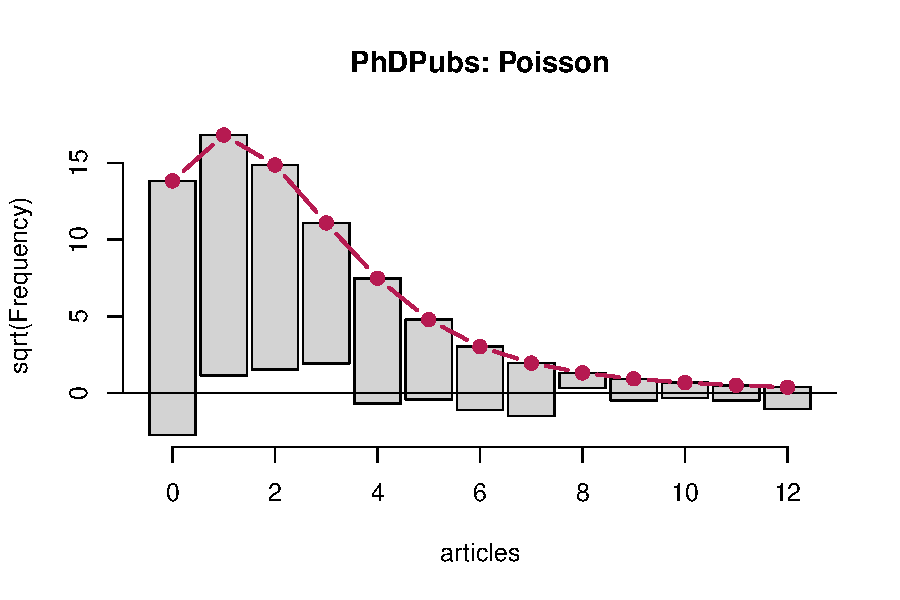
\includegraphics[width=.49\textwidth]{ch09/fig/phdpubs4-rootogram1} 
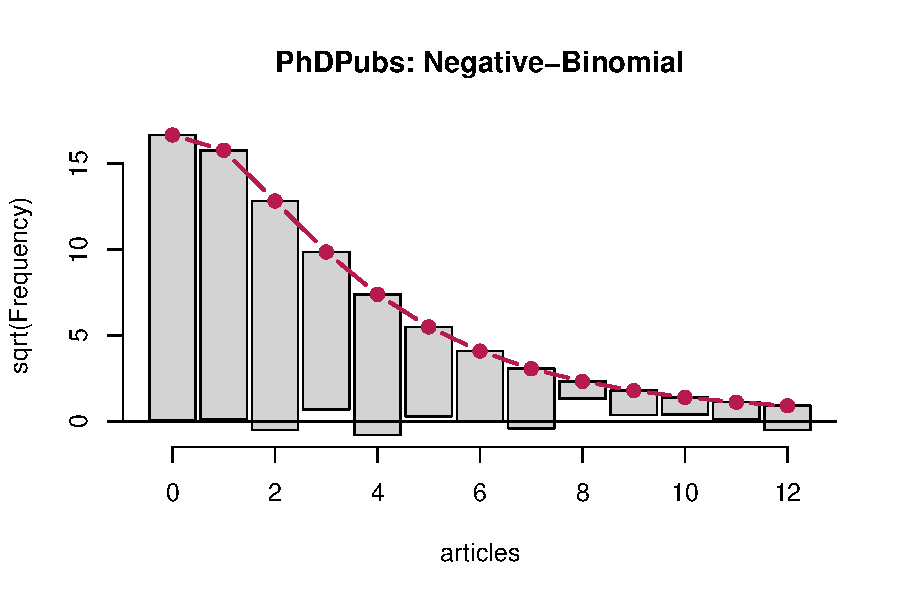
\includegraphics[width=.49\textwidth]{ch09/fig/phdpubs4-rootogram2} }

\caption[Hanging rootograms for the PhdPubs data]{Hanging rootograms for the PhdPubs data.\label{fig:phdpubs4-rootogram}}
\end{figure}


\end{knitrout}
The Poisson model shows a systematic, wave-like pattern with excess zeros, too few observed frequencies for
counts of
1--3, but generally greater frequencies for counts of 4 or more.  The negative-binomial model
clearly fits much better, though there is a peculiar tendency among the smaller
frequencies for 8 or more articles.
\end{Example}

\begin{Example}[crabs2]{Mating of horseshoe crabs}
\figref{fig:crabs2-rootogram} shows similar plots for the same two models fit to the number of
crab satellites.  The fit of the Poisson model clearly reveals the excess of zero male satellites.
For the negative-binomial, the rootogram no longer exhibits same wave-like pattern, 
however, the underfitting of the count for 0 and overfitting for counts 1--2 is 
characteristic of data with excess zeros.

\begin{knitrout}
\definecolor{shadecolor}{rgb}{1, 0.961, 0.933}\color{fgcolor}\begin{kframe}
\begin{alltt}
\hlstd{countreg::}\hlkwd{rootogram}\hlstd{(crabs.pois,} \hlkwc{max}\hlstd{=}\hlnum{15}\hlstd{,} \hlkwc{main}\hlstd{=}\hlstr{"CrabSatellites: Poisson"}\hlstd{)}
\hlstd{countreg::}\hlkwd{rootogram}\hlstd{(crabs.nbin,} \hlkwc{max}\hlstd{=}\hlnum{15}\hlstd{,} \hlkwc{main}\hlstd{=}\hlstr{"CrabSatellites: Negative-Binomial"}\hlstd{)}
\end{alltt}
\end{kframe}\begin{figure}[!htbp]


\centerline{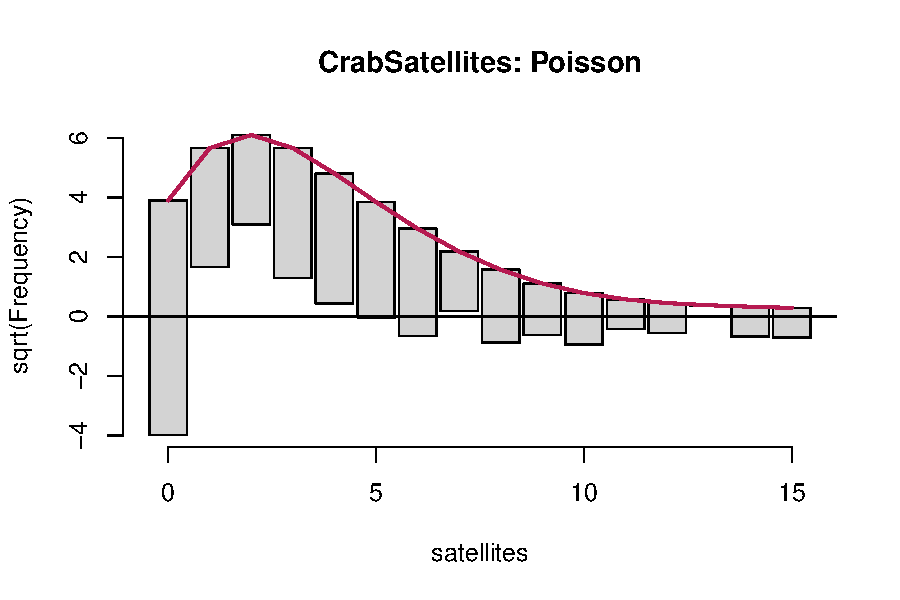
\includegraphics[width=.49\textwidth]{ch09/fig/crabs2-rootogram1} 
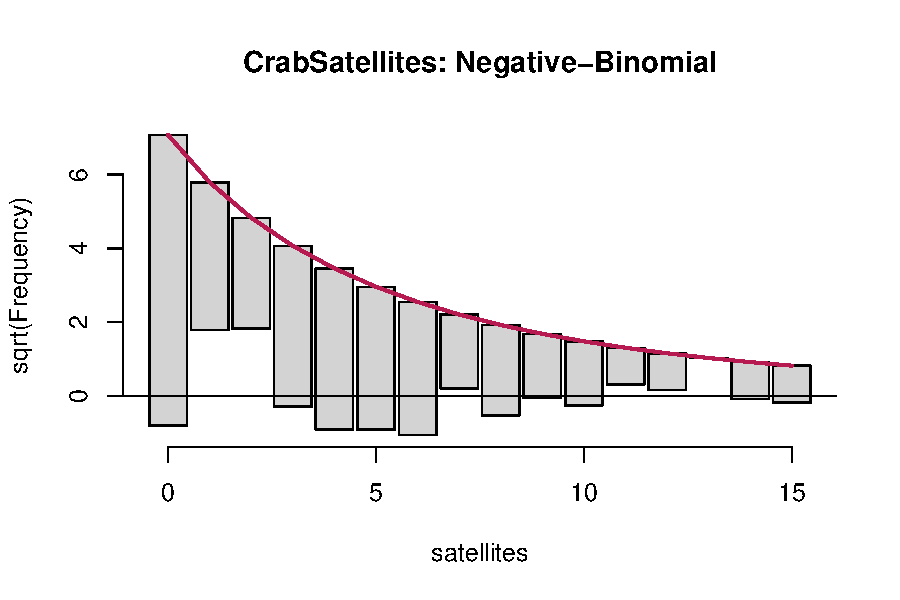
\includegraphics[width=.49\textwidth]{ch09/fig/crabs2-rootogram2} }

\caption[Hanging rootograms for the CrabSatellites data]{Hanging rootograms for the CrabSatellites data.\label{fig:crabs2-rootogram}}
\end{figure}


\end{knitrout}
\end{Example}



\section{Models for excess zero counts}\label{sec:glm-zeros}

%\section{Models for excess zero counts}\label{sec:glm-zeros}

In addition to overdispersion, many sets of empirical data exhibit a greater prevalence of
zero counts than can be accommodated by the Poisson or negative-binomial models.
We saw this in the \data{PhdPubs} data set, where there were many candidates who had
not published at all, and in the \data{CrabSatellites} data where a large number of
females attracted no unattached males.
Other examples abound in many different fields: studies of the 
use of health care services often find that many people never visit a hospital
in some time frame; similarly, the distribution of insurance claims often shows
large numbers who make no claims \citep{YipYau:2005} because of under-reporting
of small claims, policy deductible provisions and desire to avoid premium increases.


Beyond simply identifying this as a problem of lack-of-fit,
understanding the reasons for excess zero counts can make a contribution to a
more complete explanation of the phenomenon of interest,
and this requires both new statistical models and visualization techniques
illustrated in this section.

In the first example, \citet{Long:1997} argued that the PhD candidates might fall into
two distinct groups: ``publishers'' (perhaps striving for an academic career)
and ``non-publishers'' (seeking other career paths).  Of the 275 observations
having \code{articles==0}, some might not have published due to chance or
unmeasured factors.  One reasonable form of explanation is that the observed
zero counts reflect a mixture of the two latent classes--- those who simply
have not yet published and those who will likely never publish.
A statistical formulation of this idea leads to the class of \emph{zero-inflated}
models described below.

A different form of explanation is that there may be some special 
circumstance or ``hurdle'' required to achieve a positive count,
like publishing the master's thesis
(such as being driven internally by a personality trait or externally by
pressure from a mentor). This idea leads to the class of \emph{hurdle} models
that entertain and fit (simultaneously) two separate models: one for the
occurrrence of the zero counts, and one for the positive counts.

\subsection{Zero-inflated models}\label{sec:glm-zip}

Zero-inflated models, introduced by \citet{Lambert:1992} as the \term{zero-inflated Poisson}
(ZIP) model, provide an attractive solution to the problem of dealing with an overabundance of
zero counts.  It postulates that the observed counts arise from a mixture of two latent classes
of observations: some structural zeros for whom $y_i$ will always be 0, and the rest, sometimes
giving random zeros.
The ZIP model is comprised of two components:
\begin{itemize}
  \item A model for the binary event of membership in the unobserved (latent) class of
  those for whom the count is necessarily zero (e.g., ``non-publishers'').  
  This is typically taken as a logistic regression for the probability $\pi_i$ that
  observation $i$ is in this class, with predictors $\vec{z}_1, \vec{z}_2, \dots, \vec{z}_q$, giving
\begin{equation}\label{eq:zip-logit}
 \logit (\pi_i) = \vec{z}_i\trans \vec{\gamma}
                = \gamma_0 + \gamma_1 z_{i1} + \gamma_2 z_{i2} + \cdots + \gamma_q z_{iq} \period
\end{equation}

  \item A Poisson model for the other class (e.g., ``publishers''), for whom the observed count may 0 or
  positive. This model typically uses the usual log link to predict the mean, using predictors
  $\vec{x}_1, \vec{x}_2, \dots, \vec{x}_p$, so
\begin{equation}\label{eq:zip-pois}
  \log_e  \: \mu (\vec{x}_i) = \vec{x}_i \trans \vec{\beta}
                 = \beta_0 + \beta_1 x_{i1} + \beta_2 x_{i2} + \cdots + \beta_q x_{ip} \period
\end{equation}
\end{itemize}
In application, it is permissible and not uncommon to use the same set of predictors
$x = z$ in both submodels, but the notation indicates that this is not required.
Some simple special cases arise when the model for the always zero latent class
is an intercept-only model, $\logit (\pi_i) = \gamma_0$, implying the same probability
for all individuals, and (less commonly) when the Poisson mean model is intercept-only
with no predictors but there might be excess zero counts.

With this setup, one can show that the probability of observing counts of $y_i = 0$
and $y_i > 0$ are
\begin{eqnarray}
\Pr ({y_i} = 0 \given \vec{x}, \vec{z}) &=& {\pi _i} + (1 - {\pi _i}){e^{ - {\mu _i}}} \label{eq:zip-probs} \\
\Pr ({y_i} \given \vec{x}, \vec{z}) &=& (1 - {\pi _i}) \times \left[\frac{{{\mu _i}^{{y_i}}{e^{ - {\mu _i}}}}}{{{y_i}!}} \right] \comma \quad\quad y_i \ge 0 \nonumber
\end{eqnarray}
where the term in brackets in the second equation is the Poisson probability $\Pr(y=y_i)$
with rate parameter $\Pois(\mu_i)$. In these equations, 
$\pi_i= \logit^{-1} (\vec{z}_i\trans \vec{\gamma}) $ depends on the $\vec{z}$ through \eqref{eq:zip-logit}, and 
$\mu_i = \exp(\vec{x}\trans\vec{\beta})$ depends on the $\vec{x}$
through \eqref{eq:zip-pois}.

The conditional expectation and variance of $y_i$ then have the forms
\begin{eqnarray*}
\E (y_i) &=& (1 - {\pi _i}) \: \mu_i  \\
\V (y_i) &=& (1 - {\pi _i}) \: \mu_i  (1 + \mu_i \pi_i ) \period
\end{eqnarray*}
Thus, when $\pi_i > 0$, the mean of $y$ is always less than $\mu_i$,
and the variance of $y$ is greater than its mean by a dispersion factor of $(1 + \mu_i \pi_i)$.

There is nothing special about the use of the Poisson distribution here. The model for the
count variable could also be taken as the negative-binomial, giving a
\emph{zero-inflated negative-binomial} (ZINB) model using $\NBin (\mu, \theta)$ or
a \emph{zero-inflated geometric} model using $\NBin (\mu, \theta=1)$.

There are several packages in \R capable of fitting zero-inflated models.  The most mature and
complete of these is \func{zeroinfl} in 
the \Rpackage{countreg} (a successor to the \Rpackage{pscl})
The function \func{zeroinfl} is modeled after \func{glm}, but provides an extended syntax
for the model formula.

If the \code{formula} argument is supplied in the form
\verb|y ~ x1 + x2 + ...|, it not only describes the count regression of $y$ on
$x_1, x_2, \dots$, but also implies that the \emph{same} set of regressors, $z_j = x_j$,
is used for the zero count binary submodel.  The extended syntax  uses the
notation 
\verb#y ~ x1 + x2 + ... | z1 + z2 + ...# 
to specify the $x$ variables separately, conditional on (\code{|})
the always-zero count model \verb|y ~ z1 + z2 + ...|.
The model for the not-always-zero class can be specified using the
\code{dist} argument, with possible values
\code{"poisson"}, \code{"negbin"} and \code{"geometric"}.


\subsection{Hurdle models}\label{sec:glm-hurdle}
A different class of models capable of accounting for excess zero counts is the 
\term{hurdle model} proposed initially by \citet{Cragg:1971} and developed further by
\citet{Mullahy:1986}.
This model also uses a separate logistic regression submodel to distinguish
counts of $y=0$ from larger counts, $y>0$.
The submodel for the positive counts is expressed as a (left) \emph{truncated}
Poisson or negative-binomial model, excluding the zero counts.
As an example, consider a study of behavioral health in which one outcome is
the number of cigarettes smoked in one month.  All the zero counts will come from
non-smokers and smokers will nearly always smoke a positive number.

This differs from the set of ZIP models in that classes of $y=0$ and $y>0$
are now considered fully-observed, rather than latent.
Conceptually, there is one process and submodel acounting for the zero counts
and a separate process accounting for the positive counts, once the ``hurdle''
of $y=0$ has been passed.
In other words, for ZIP models, the first process generates 
only extra zeros beyond those of the regular Poisson distribution. 
For hurdle models, the first process generates all of the zeros.
The probability equations corresponding to \eqref{eq:zip-probs} are:
\begin{eqnarray}
\Pr ({y_i} = 0 \given \vec{x}, \vec{z}) &=& {\pi _i} \\
\Pr ({y_i} \given \vec{x}, \vec{z}) &=& \frac{(1 - {\pi _i})}{1-e^{-\mu_i}} 
\times \left[\frac{{{\mu _i}^{{y_i}}{e^{ - {\mu _i}}}}}{{{y_i}!}} \right] \comma \quad\quad y_i \ge 0 \nonumber
\end{eqnarray}
% and the mean regression relationship can be expressed as
% \begin{equation*}
%  \log_e  \: \mu (\vec{x}_i) = \vec{x}_i \trans \vec{\beta}
%           + log_e (1 - \pi_i) - log_e(1 - ) 
% \end{equation*}

The hurdle model can be fitted in \R using the \func{hurdle} function from the \Rpackage{countreg}.
The syntax for the model formula is the same extended form provided by \func{zeroinfl},
where \verb|y ~ x1 + x2| uses the same regressors for the zero and positive count submodels,
while \verb#y ~ x1 + x2 | z1 + z2# uses \verb|y ~ z1 + z2| for the zero hurdle model.
Similarly, the count distribution can be given 
as 
\code{"poisson"}, \code{"negbin"} or \code{"geometric"}
with the \code{dist} argument.  For \func{hurdle}, the distribution for zero model
can be specified with a \code{zero.dist} argument. The default is \code{"binomial"}
(with a logit \code{link}), but other right-censored
distributions can also be specified.

\subsection{Visualizing zero counts}\label{sec:glm-viszero}

Both the zero-inflated and hurdle models treat the zero counts $y=0$ specially with separate
submodels, so the binary event of $y=0$ vs.\ $y>0$ can be visualized using any of the techniques
illustrated in \chref{ch:logistic}.  See \secref{sec:logist-plotting}, \secref{sec:logist-condplots}
and \secref{sec:logist-fullplots} for some examples that plot both the binary observations
and a model summary or smoothed curve to show the relationships with one or more
regressors.  To apply these ideas in the current context, simply define or plot a logical
variable corresponding to the expression \code{y==0}, giving values of \code{TRUE} or \code{FALSE}.

A different, and simpler idea is illustrated here using what is called a \term{spine plot}
\cite{Hummel:96} when a predictor $x$ is a discrete factor or \term{spinogram} when $x$ is
continuous.  Both are forms of mosaic plots with special formatting of spacing and shading,
and in this context they plot $\Pr(y=0 | x)$ against $\Pr(x)$; when $x$ is numerical, it
is first made discrete, as in a histogram. 
Then, in the spine plot or spinogram, the widths of the bars correspond to the relative frequencies of $x$
and heights of the bars correspond to the conditional relative frequencies of $y=0$ in every $x$ group. 
In \R, spine plots are implemented in the function \func{spineplot}, however, this is what you
get by default if you use \verb|plot(y==0 ~ x)| to plot the binary factor against any regressor $x$.

A related graphical method is the \term{conditional density plot}
\citep{HofmannTheus:2005}. The conditional probabilities $\Pr(y=0 | x)$ are derived using
a smoothing approach (via \func{density}) over $x$ rather than by making $x$ discrete.
These plots are provided by \func{cdplot} in the \Rpackage{graphics} and a similar
\func{cd\_plot} in \pkg{vcd}.  The smoothing method for the density estimate is controlled
by a \code{bw} (bandwith) method and other arguments.

\begin{Example}[crabs-zero]{Mating of horseshoe crabs}
For the \data{CrabSatellites} data, we can examine the relationship of the zero counts
(females who attract no unattached male satellites) to the predictors using spinograms
or conditional density plots.  Here, we consider \var{weight} and \var{color} (treated numerically) as
predictors. \TODO{Fixup use of color in \exref{ex:crabs1} so it doesn't cause a problem here}




\begin{knitrout}
\definecolor{shadecolor}{rgb}{1, 0.961, 0.933}\color{fgcolor}\begin{kframe}
\begin{alltt}
\hlstd{op} \hlkwb{<-} \hlkwd{par}\hlstd{(}\hlkwc{cex.lab}\hlstd{=}\hlnum{1.2}\hlstd{,} \hlkwc{mfrow} \hlstd{=} \hlkwd{c}\hlstd{(}\hlnum{1}\hlstd{,} \hlnum{2}\hlstd{))}
\hlkwd{plot}\hlstd{(}\hlkwd{factor}\hlstd{(satellites} \hlopt{==} \hlnum{0}\hlstd{)} \hlopt{~} \hlstd{weight,} \hlkwc{data} \hlstd{= CrabSatellites,}
     \hlkwc{breaks} \hlstd{=} \hlkwd{quantile}\hlstd{(weight,} \hlkwc{probs}\hlstd{=}\hlkwd{seq}\hlstd{(}\hlnum{0}\hlstd{,}\hlnum{1}\hlstd{,}\hlnum{.2}\hlstd{)),} \hlkwc{ylevels}\hlstd{=}\hlnum{2}\hlopt{:}\hlnum{1}\hlstd{,}
     \hlkwc{ylab}\hlstd{=}\hlstr{"No satellites"}\hlstd{)}
\hlkwd{plot}\hlstd{(}\hlkwd{factor}\hlstd{(satellites} \hlopt{==} \hlnum{0}\hlstd{)} \hlopt{~} \hlstd{color,} \hlkwc{data} \hlstd{= CrabSatellites,}
     \hlkwc{breaks} \hlstd{=} \hlkwd{quantile}\hlstd{(color,} \hlkwc{probs}\hlstd{=}\hlkwd{seq}\hlstd{(}\hlnum{0}\hlstd{,}\hlnum{1}\hlstd{,}\hlnum{.33}\hlstd{)),}  \hlkwc{ylevels}\hlstd{=}\hlnum{2}\hlopt{:}\hlnum{1}\hlstd{,}
     \hlkwc{ylab}\hlstd{=}\hlstr{"No satellites"}\hlstd{)}
\hlkwd{par}\hlstd{(op)}
\end{alltt}
\end{kframe}\begin{figure}[!htbp]


\centerline{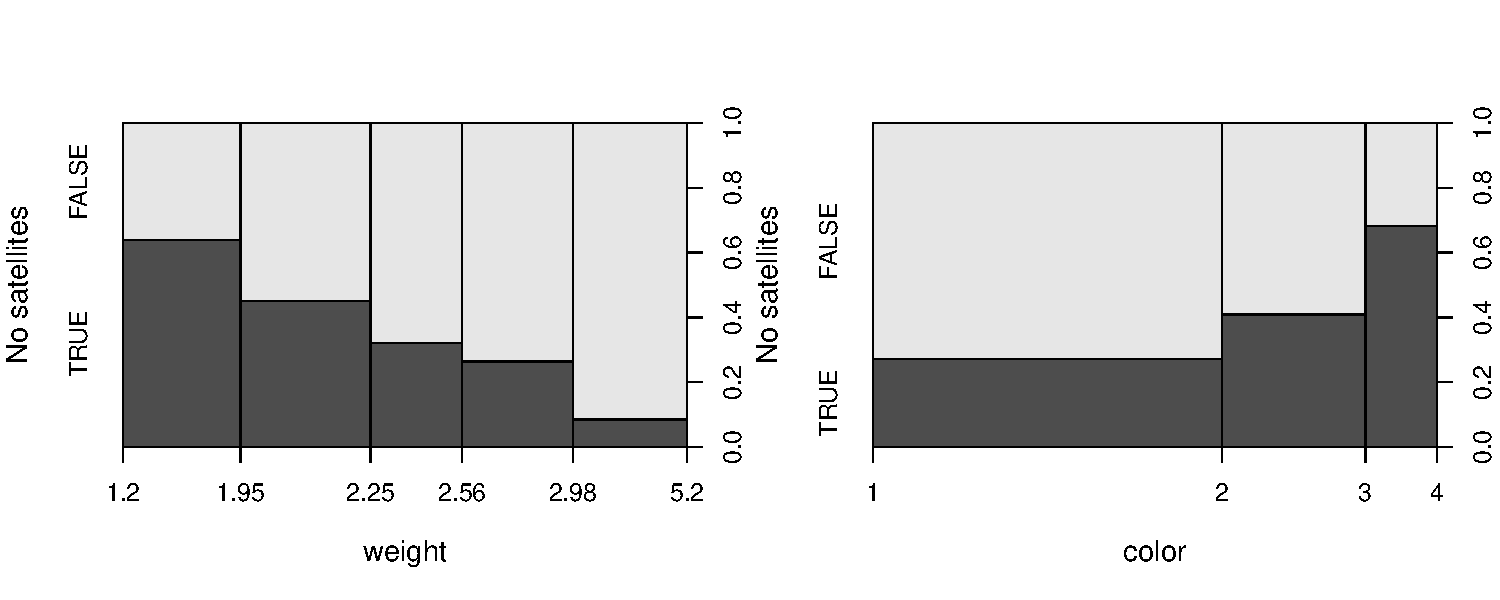
\includegraphics[width=\textwidth]{ch09/fig/crabs-zero-spinogram} }

\caption[Spinograms for the CrabSatellites data]{Spinograms for the CrabSatellites data. The variables weight (left) and color(right) have been made discrete using quantiles of their distributions.\label{fig:crabs-zero-spinogram}}
\end{figure}


\end{knitrout}

\begin{knitrout}
\definecolor{shadecolor}{rgb}{1, 0.961, 0.933}\color{fgcolor}\begin{kframe}
\begin{alltt}
\hlstd{op} \hlkwb{<-} \hlkwd{par}\hlstd{(}\hlkwc{cex.lab}\hlstd{=}\hlnum{1.2}\hlstd{,} \hlkwc{mfrow} \hlstd{=} \hlkwd{c}\hlstd{(}\hlnum{1}\hlstd{,} \hlnum{2}\hlstd{))}
\hlkwd{cdplot}\hlstd{(}\hlkwd{factor}\hlstd{(satellites} \hlopt{==} \hlnum{0}\hlstd{)} \hlopt{~} \hlstd{weight,} \hlkwc{data} \hlstd{= CrabSatellites,}
       \hlkwc{ylevels}\hlstd{=}\hlnum{2}\hlopt{:}\hlnum{1}\hlstd{,} \hlkwc{ylab}\hlstd{=}\hlstr{"No satellites"}\hlstd{)}
\hlkwd{cdplot}\hlstd{(}\hlkwd{factor}\hlstd{(satellites} \hlopt{==} \hlnum{0}\hlstd{)} \hlopt{~} \hlstd{color,} \hlkwc{data} \hlstd{= CrabSatellites,}
       \hlkwc{ylevels}\hlstd{=}\hlnum{2}\hlopt{:}\hlnum{1}\hlstd{, ,} \hlkwc{ylab}\hlstd{=}\hlstr{"No satellites"}\hlstd{)}
\hlkwd{par}\hlstd{(op)}
\end{alltt}
\end{kframe}\begin{figure}[!htbp]


\centerline{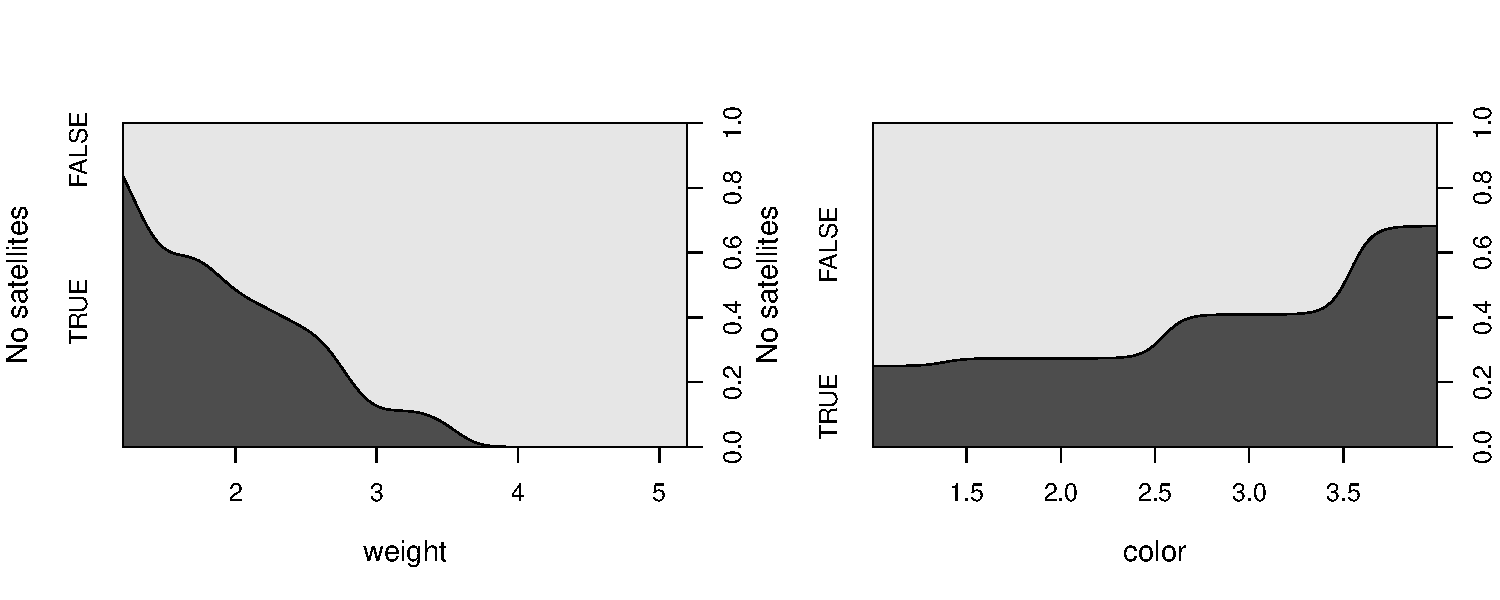
\includegraphics[width=\textwidth]{ch09/fig/crabs-zero-cdplot} }

\caption[Conditional density plots for the CrabSatellites data]{Conditional density plots for the CrabSatellites data. The region shaded below shows the conditional probability density estimate for a count of zero.\label{fig:crabs-zero-cdplot}}
\end{figure}


\end{knitrout}


\end{Example}

%\subsection{Zero-inflated models}\label{sec:glm-zip}
%\subsection{Hurdle models}\label{sec:glm-hurdle}


\section{Diagnostic plots for model checking}\label{sec:glm-diag}

\section{Chapter summary}

\section{Further reading}

\section{Lab exercises}

% Cleanup local variables
\begin{knitrout}\footnotesize
\definecolor{shadecolor}{rgb}{1, 0.961, 0.933}\color{fgcolor}\begin{kframe}
\begin{alltt}
\hlcom{# detach(package:ggtern)  ## detach any masking packages}
\hlstd{.locals}\hlopt{$}\hlstd{ch09} \hlkwb{<-} \hlkwd{setdiff}\hlstd{(}\hlkwd{ls}\hlstd{(), .globals)}
\hlstd{.locals}\hlopt{$}\hlstd{ch09}
\end{alltt}
\begin{verbatim}
##  [1] "art.fac"         "art.tab"         "blogits"        
##  [4] "crabs.nbin"      "crabs.nbin1"     "crabs.pois"     
##  [7] "crabs.pois1"     "CrabSatellites"  "CrabSatellites1"
## [10] "cutfac"          "cutq"            "fit.nbin"       
## [13] "fit.pois"        "group"           "interp"         
## [16] "knitrSet"        "logi.hist.plot"  "logit2p"        
## [19] "LRtest"          "op"              "phd.nbin"       
## [22] "phd.pois"        "phd.qpois"       "PhdPubs"        
## [25] "phi"             "print_coef"      "pun_cotab"      
## [28] "qdat"            "spar"
\end{verbatim}
\begin{alltt}
\hlkwd{remove}\hlstd{(}\hlkwc{list}\hlstd{=.locals}\hlopt{$}\hlstd{ch09[}\hlkwd{sapply}\hlstd{(.locals}\hlopt{$}\hlstd{ch09,}\hlkwa{function}\hlstd{(}\hlkwc{n}\hlstd{)\{}\hlopt{!}\hlkwd{is.function}\hlstd{(}\hlkwd{get}\hlstd{(n))\})])}
\end{alltt}
\end{kframe}
\end{knitrout}



%%%%%%%%%%%%%%%%%%%%%%%%%%%%%%%%%%%%%%%%%%%%%%%%%%%%%%%%%%%%%%%%%%%%%%%%%


% To resolve citations in the chapter, ...
{\itemsep -1pt
\bibliography{graphics,statistics,timeref,Rpackages}
%%% Use aux2bib to process the .aux file, creating references.bib
%%% Then change to line below
%\bibliography{references}
}

% \newpage
% This document was produced using:
% 
% <<session-info>>=
% print(sessionInfo(), locale = FALSE)
% @

	
%%%%% THE END %%%%%
\end{document}

